\documentclass{amsart}[12pt]
\usepackage{longtable, latexsym, amsmath, amsfonts, tikz}
\usepackage{natbib}
\oddsidemargin=0in \evensidemargin=0in
\textwidth=6.6in \textheight=8.7in

\tikzset{
chamber1/.pic={
  \draw[dotted] (0, 0) -- (0.85,1.5) -- (1.7, 0) -- (0, 0) ;
  \draw (0, 0) circle [radius=0.05] node[anchor=south] {\tiny A};
  \draw (0.85, 1.5) circle [radius=0.05] node[anchor=west] {\tiny C};
  \draw (1.7, 0) circle [radius=0.05] node[anchor=south] {\tiny B};
  },
chamber2/.pic={
\draw[dotted] (0,1) -- (1,0) -- (2,1) -- (1,2) -- (0,1);
\draw[dotted] (0,1) -- (2,1);
\draw (0,1) circle [radius=0.05] node[anchor=south] {\tiny A};
\draw (1,0) circle [radius=0.05] node[anchor=west] {\tiny C};
\draw (2,1) circle [radius=0.05] node[anchor=south] {\tiny B};
\draw (1,2) circle [radius=0.05] node[anchor=west] {\tiny C};
  },
chamber4/.pic={
  \draw[dotted] (0,1) -- (1,0) -- (2,1) -- (1,2) -- (0,1);
  \draw[dotted] (0,1) -- (2,1);
  \draw[dotted] (1,0) -- (1,2);
  \draw (0,1) circle [radius=0.05];
  \draw (1,0) circle [radius=0.05];
  \draw (2,1) circle [radius=0.05];
  \draw (1,2) circle [radius=0.05];
  }
}

\title{Operations on polyhedra}
\author{B R S Recht}
\date{July 2018}


\begin{document}

\maketitle

The motivations for this line of inquiry are:
\begin{itemize}
  \item Classification. The inflation factor introduced in Brinkmann et
  al. \cite{brinkmann} is a good measure of the complexity of certain operators.
  Are there more invariants that can be used to classify operators?
  \item Relationships between operators. How can operators be composed? How can
  an operator be decomposed into other operators?
\end{itemize}

\section{Definitions}

An abstract polytope $P$ is a ranked poset satisfying the properties below.
Elements of rank $0$ may be called vertices; of rank $1$, edges; of rank $2$,
faces. (In most literature on abstract polytopes all elements of the poset are
called (abstract) faces, but since this work is primarily concerned with
polyhedra, it would be confusing.) The order relation $<$ on the poset
represents incidence between elements: for example, a face is incident on an
edge, which is incident on a vertex.\cite{mcmullen}
\begin{enumerate}
  \item $P$ contains a least element with rank $-1$ and a greatest
  element with rank $n$. ($n$ is the rank of the abstract polytope.)
  \item Each flag of $P$ has the same length and includes the least and greatest
  elements. (A flag is a series of incident elements from the least element to
  the greatest)
  \item $P$ is strongly connected: any flag can be changed into any other flag
  by changing one element of the flag at a time.
  \item $P$ satisfies the diamond property: if an element $A$ has rank $k-1$,
  and an element $C$ has rank $k+1$, there are exactly $2$ elements $B$ of
  rank $k$ such that $A < B < C$.
\end{enumerate}
Occasionally a structure that violates one of these properties may be useful;
these will be discussed as they appear. The skeleton of a polytope is the
(possibly multi-) graph formed by its vertices and edges.
The dual of an abstract polytope is simply the abstract polytope with its order
and rank reversed. (This corresponds to the usual geometric notion of dual.)

The $f$-vector of a polytope is the vector of counts of elements of each rank.
Normally the greatest and least elements are omitted (since they're always 1),
and the vector has the form $(a_0, \ldots, a_{d-1})$ where $a_i$ is the count
of elements of rank $i$. The extended $f$-vector includes those elements:
$(a_{-1}=1, a_0, \ldots, a_{d-1}, a_d=1)$. The vector is half-extended if
only one of those endpoints is included. As such, the (extended) $f$-vector of
the dual of a polytope is the (extended) $f$-vector of the original polytope,
reversed. The $f$-polynomial is $F(x) = \sum_{i=-1}^d a_i x^{i+1}$.
The Euler characteristic of a polytope is the alternating
sum of the elements of the $f$-vector: $\chi = a_0 - a_1 + a_2 \ldots$.

A realization of an abstract polytope is an abstract polytope $P$ mapped into
a topological space, usually, but not necessarily, $\mathbb{R}^n$. Some
realizations may be called faithful, which is not consistently defined, but
usually means that the polytope does not have self-intersections,
repeated points, digons, etc.

An abstract polyhedron $P$ is an abstract polytope of rank 3. This generalizes
things like convex polyhedra, tilings of the plane, and spherical polyhedra.
Some of the properties above have more explicit consequences for
polyhedra: \cite{grunbaum03}
\begin{itemize}
  \item Each edge is incident to 2 distinct vertices. This is the usual
  definition of edge, but here it is a consequence of earlier definitions.
  \item Each edge is incident to 2 distinct faces. This excludes things like
  space-filling honeycomb structures (where more than 2 faces may meet at an
  edge)\footnote{Honeycombs may be valid polytopes of rank 4, however.} and
  partial tilings of the plane (where fewer than 2 faces may meet at an edge).
  \item The faces may be self-intersecting, but may not contain interior holes.
\end{itemize}
The degree of a vertex is the number of edges to which it is incident. The
degree of a face is the number of edges which are incident to it, i.e. its
number of sides. (An edge of a polyhedron is always incident to 2 faces and 2
vertices, so defining degree for edges is not useful here, although it is for
higher polytopes.)
Abstract polyhedra permit faces of degree 2, called digons. Digons are
disallowed by many definitions of polyhedra, but appear in spherical polyhedra
(for example). Digons occur naturally in the study of operations on polyhedra.
The count of vertices, edges, and faces is be denoted $v, e, f$. The Euler
characteristic is $\chi = v - e + f$. The count of vertices or faces of a
certain degree is denoted $v_i$ and $f_i$ where $i$ is the degree, such that
$\sum_i v_i = v$ and $\sum_i f_i = f$.

The term polyhedron here will mean ``realization of an abstract polyhedron.''
Unless otherwise specified, polyhedra here do not require distinct vertices,
convex faces, straight edges, non-intersecting faces, flat faces, or other
things that may be required of other classes of polyhedra. This might seem
odd if you're used to standard polyhedra, but examples appear naturally: see
for example Figure \ref{fig:circlesquare}, which is a common motif in quilting.
We won't make much
use of abstract polyhedra directly, but we need them as a theoretical
underpinning. A structure that resembles a polyhedron but does not satisfy the
axioms of an abstract polytope is here called a quasipolyhedron.
\begin{figure}
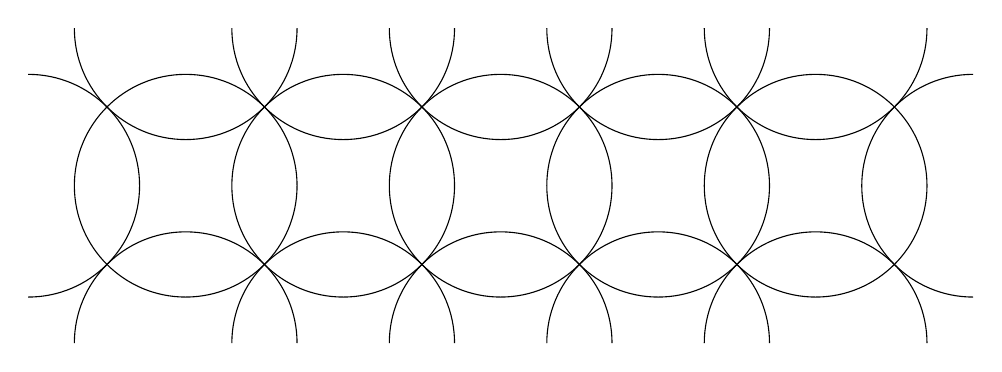
\begin{tikzpicture}
\draw (-2,-1.4142) arc [radius=1.4142, start angle=-90, end angle= 90];
\draw (10,-1.4142) arc [radius=1.4142, start angle=270, end angle= 90];
\foreach \x in {0,2,4,6,8}{
  \draw (\x,0) circle [radius=1.4142];
  \draw (-1.4142 + \x,-2) arc [radius=1.4142, start angle=180, end angle= 0];
  \draw (-1.4142 + \x,2) arc [radius=1.4142, start angle=-180, end angle= 0];
}
\end{tikzpicture}

\caption{A tiling of the plane created by overlapping circles, consisting of
digons and concave quadrilaterals with curved edges.}
\label{fig:circlesquare}
\end{figure}

An achiral polyhedron is one that has mirror symmetry: a chiral polyhedron is
one that does not. Note that the particular handedness of a chiral polyhedron
is a quality of the realization, not the underlying abstract structure.
An acoptic polyhedron is (loosely) a polyhedron that does not
self-intersect. \cite{grunbaum99} Its faces are simple polygons with straight
edges that do not self-intersect (although they may be concave). A convex
polyhedron is an acoptic polyhedron that is convex: any line between points on
the surface of the polyhedron is contained in the interior of the polyhedron.
By Steinitz's theorem, the skeleton of every convex polyhedron is a
3-vertex-connected planar graph. Furthermore, all convex polyhedra have a
realization such that each edge is tangent to the unit sphere,
each face is flat, and the centroid of the vertices lies at the origin. This is
called the canonical realization. \cite{ziegler}

An operator on polyhedra is simply a map $x : \mathcal{P} \to \mathcal{P}$,
where $\mathcal{P}$ is the set of polyhedra. Operators which break the mirror
symmetry of a polyhedron are called chiral: ones that preserve it are achiral.
We'll often apply operators to a restricted set of polyhedra, e.g. convex
polyhedra, or polyhedra with triangular faces. Sometimes we will look at maps
satisfying $x : \mathcal{X} \to \mathcal{Y}$ where $\mathcal{X}$ and
$\mathcal{Y}$ are different subsets of polyhedra: we will still call these
operators on polyhedra (instead of transformations). We'll use a calligraphic
typeface for sets of polyhedra or quasipolyhedra.

\section{Notable operations}

This section isn't a complete survey of operations on polyhedra. The concept
dates back to Kepler, and some operations have had ambiguous or changing
definitions in the past, so going through all that history would just muddy the
waters. Instead, this section summarizes some useful operators that motivate
the discussion herein or will be applied.

\subsection{Operations defined in Coxeter's Regular Polytopes}

In Coxeter's classic text \textit{Regular Polytopes}\cite{coxeter73},
he defines a handful of operations on regular polytopes:
\begin{itemize}
  \item The dual is defined in the usual way, compatible with how it was
  defined earlier in this text.
  \item Various forms of truncation are defined. The simple truncation is
  described by analogy with the polygonal case: cut off each corner of a
  polygon in such a way that the new polygon has vertices at the midpoint of
  each original edge. Other forms of truncation that retain part of the original
  edge are mentioned but not described. It is also commented that for regular
  polyhedra, the truncation is equivalent to the intersection
  of the (canonical realization of) the original polyhedra and its dual.
  \item An operation, partial truncation or alternation, is defined on regular
  polytopes with even-degree faces. Alternating vertices are cut off or
  retained. This results in digons for degree-4 faces,
  which are treated as edges.
  \item The snub operation (different than Conway's snub)
  is equivalent to simple truncation followed by alternation.
\end{itemize}

Coxeter's construction of simplexes can be cast in terms of abstract polyhedra.
Simply take the poset direct product of a number of copies of the unique
abstract polyhedron of rank 1 (a single point). The product of two points is an
edge: of three, a triangle, of four, a tetrahedron, and so on. This can be
thought of as a binary operation on simplexes, so e.g. the product of two edges
is a tetrahedron. (Also, suggestively, the $f$-polynomial of a direct product
of posets is the product of the $f$-polynomial of each poset.)

\subsection{Conway's operations}
Conway described a set of operations on polyhedra and a notation for describing
those operations, with the intent of creating a systematic naming scheme for
polyhedra.\cite{conway} He used a prefix notation, where the rightmost element
is a polyhedral seed and operators apply from right to left. Each operator is
assigned a letter and a name. So, for instance, $dO$ is the dual of a regular
octahedron (i.e. a cube), and $taO$ is a truncated ambo octahedron, more
commonly known as the truncated cuboctahedron. Conway's original set of
operations is denoted with the letters $abdegjkmost$: a full list of their
descriptions will be given later. These operations are sufficient to create all
of the Archimedean and Catalan solids from the Platonic solids. Others have
defined more operations. \cite{hart98}\cite{hart00}\cite{antiprism}
In particular, Hart \cite{hart98} defined $r$,
which reverses the chirality of a polyhedra.

Aside from $g, s, j$, and $a$, Conway's operations preserve the
symmetry of the resultant polyhedra. $g$ and $s$ are achiral, so
do not preserve mirror symmetry. $j$ and $a$ actually increase
the symmetry: in fact, it is possible to express the other 4 Platonic solids
in terms of the tetrahedron $T$ using $j$ and $a$.

Some of Conway's operations can be expressed in terms of other operations:
$e=aa, o=jj, m=kj$, and $b=ta$. Borrowing an idea from ring
theory, we refer to $d$ (dual) and $S$ (seed, identity) as the
units of the EROs, and operators that are related by $d$ are called
associates. At most 4 operators can be associated with each other, corresponding
to $x$, $xd$, $dx$, and $dxd$.
Conway's operators are associated as so:

\begin{itemize}
  \item $j=jd, a=dj=djd$
  \item $k, t=dkd$ (as well as $n=kd$ and $z=dk$)
  \item $o=od, e=do=dod$
  \item $g, s=dgd$ (as well as $rgr=gd$ and $rsr=sd$)
  \item $m=md, b=dm=dmd$
\end{itemize}

Some Conway operators have an indexed form that indicates that only certain faces or
vertices are operated on. For instance, $k_i$ applies kis to faces with
$i$ sides, and $t_i$ truncates vertices of degree $i$.
Operations like this do not in general preserve the symmetry of the seed
polyhedron.

\subsection{Goldberg-Coxeter operations}
The Goldberg-Coxeter operation (GC operation) was defined by Deza and
Dutour \cite{dutour}, based on the Goldberg polyhedra, the viral capsid
structure defined by Coxeter \cite{coxeter71}, the geodesic domes of Buckminster
Fuller, and similar structures. Essentially it amounts to replacing the faces of
a polyhedra with a section from a grid of triangular or square faces. Here the
operation on triangle-faced polyhedra will be denoted $\Delta_{a,b}$, and on
quadrilateral-faced polyhedra $\Box_{a,b}$, where $a$ and $b$ are integers,
$a > 0$, and $b \ge 0$.

$\Delta_{a,b}$ can be described using the triangular lattice over the
Eisenstein integers. It is useful for this operation to parameterize the
Eisenstein integers as $x = a + bu$ where $u = \frac{1}{2}(1 + i\sqrt 3) =
e^{\pi i/3}$, for reasons to be explained later. Take the section of the grid
inside the triangle with vertices $0, x(2-u)/3, x, x(1+u)/3$.

$\Box_{a,b}$ can be described using the triangular lattice over the Gaussian
integers, $x = a + bi$ where $i = \sqrt{-1}$. Take the section of the grid
inside the square with vertices $0, x(1-i)/2, x, x(1+i)/2$.

Each operator has an invariant $g$, equivalent to $g = |x|^2$. For
$\Delta_{a,b}$, $g = a^2 + b^2$: for $\Box_{a,b}$, $g = a^2 + ab + b^2$. This
can be used to calculate the count of elements in the resulting polyhedron
based on the count of elements in the original polyhedron. (The actual formula
will be shown later in a more general form.)

Two elements of the Eisenstein integers $x$ and $y$ are associates if
$y = u^n x$ for some $n$. Similarly, two elements of the Gaussian integers are
associates if $y = i^n x$ for some $n$. The associated element with $a>0$ and
$b\ge 0$ is the normal form. (We use the alternate definition for Eisenstein
integers so that the same definition for normal form applies to both operators.
This is also the traditional definition used by Goldberg polyhedra, geodesic
domes, viral capsids, etc.) Iff $e+fu$ is associated with $(a+bu)(c+du)$, then
$\Delta_{a,b}\Delta_{c,d} = \Delta_{e,f}$, and similarly for $\Box_{a,b}$.

Another consequence of the relationship between these operators and the
Eisenstein and Gausssian integers is that these operators are commutative and
associative: $\Delta_{a,b}\Delta_{c,d} = \Delta_{c,d}\Delta_{a,b}$, and
similarly for $\Box_{a,b}$. Furthermore, the Eisenstein and Gaussian integers
are Euclidean domains, which means elements of the domains can be factored
uniquely (if not irreducible), and there is a straightforward way to do so
using an extension of the Euclidean algorithm. (The invariant $g$ is the
Euclidean function in the Euclidean algorithm.)

These operators are divided into three classes.
\begin{itemize}
  \item Class I: $b = 0$, achiral
  \item Class II: $a = b$, achiral
  \item Class III: All others, chiral
\end{itemize}
All Class II operators can be reduced as
$\Delta_{a,a} = \Delta_{1,1}\Delta_{a,0}$ (and possibly further).

\subsection{Operations in the software package Antiprism}

The software package Antiprism \cite{antiprism} includes a number of
applications that perform operations on polyhedra. (Among other things, it
contains an implementation of Conway operations.) One caveat: The file format
used by antiprism, OFF, consists of a list of vertex positions and a list of
faces that references the list of vertices. This is not a fully faithful
representation of a polyhedra, as it does not contain explicit incidence
information. Problems show up for overlapping faces and digons. Digons are
referred to as explicit edges by antiprism.

Of particular interest is the application \texttt{wythoff}, in which a notation
for operations on polyhedra is introduced. Despite the name, the new notation is
much more flexible than Wythoff notation.
\texttt{wythoff} requires a polyhedron with only triangular faces, where the
vertices of the polyhedron can be 3-colored. As a consequence, the vertices must
have even order, and the faces are 2-colorable. The colored faces are labeled
$+$ or $-$. We'll call this set of polyhedra $\mathcal{W}$. \texttt{wythoff}
automatically applies Conway's meta operation to produce a polyhedron in
$\mathcal{W}$. The meta operation retains the original vertices and adds a
vertex at the center of each edge and each face. Respectively, these are labeled
$V$, $E$, and $F$. If a polyhedron is in $\mathcal{W}$ it can be used directly:
the labeling of vertices uses the same letters VEF. This is somewhat confusing since E and F no longer relate to edges or faces, so alternately the vertices
can be labeled ABC.

For example, this is the string that it uses to implement Conway's kis
operation: \texttt{[F, V] 0\_1v1v, 1E}. The extended Wythoff notation comprises
two parts. The first part, in brackets, defines points on each triangular face
using barycentric coordinates. Each point is specified as \texttt{aVbEcF}, where
\texttt{a}, \texttt{b}, and \texttt{c} are numbers. If any of those are 1, the
number may be left off: if 0, the component may be left off. So in the above,
it defines two points, more explicitly as \texttt{0V0E1F} and \texttt{1V0E0F}:
a point at vertices labeled $F$, and a point at vertices labeled $V$.

The second part defines faces as paths between these points. A \texttt{+},
\texttt{-}, or \texttt{*} at the start of a path denotes which triangle to
start with: if none, then \texttt{+} is assumed. An underscore indicates
remaining on the same triangle. A lowercase \texttt{v}, \texttt{e}, or
\texttt{f} indicates that the path crosses the edge opposite of the vertex
labelled $V$, $E$, or $F$. An uppercase \texttt{V}, \texttt{E}, or \texttt{F}
indicates a rotation by two triangles about the vertex labeled $V$, $E$, or $F$:
explicitly, these are shorthands for \texttt{ef}, \texttt{fv}, and \texttt{ve}
respectively. The first path starts at point 0 on + triangles, moves to point 1
on the same triangle, then moves over the edge opposite $V$ to point 1 on
that triangle. It then moves back over the edge and completes the path at 0
on the original triangle. (The second produces an explicit edge, and is needed
so that the operation produces a polyhedron when applied directly to a
polyhedron in $\mathcal{W}$.)

This notation is capable of representing many operations on polyhedra,
including all of Conway's operators. Notation to create the regular hemihedra
from the Platonic solids exists, as does notation to create hollowed-out,
da Vinci-style renderings of polyhedra.
It is also capable of producing quasipolyhedra.

\section{Smoothing}

Digons can be present in a faithful realization of a polyhedron, such as in
Figure \ref{fig:circlesquare}, or spherical hosohedra. However, many subsets of
polyhedra exclude digons. Degree-2 vertices are also problematic, being dual to
digons. These elements can be eliminated in a systematic manner. We define a
smoothing operator, $\$$, that transforms digons into single edges and handles
degree-2 vertices by removing that vertex and merging the vertex's incident
edges, as depicted in figure \ref{fig:smooth}. This is similar to the topic of
homeomorphism in graph theory: see \cite{ziegler} for context. Antiprism effectively smooths digons
automatically by treating them as "explicit edges".

\begin{figure}
\begin{tikzpicture}
\draw (0,0) -- (0,2);
\draw (0,1) -- (3,1);
\draw (3,0) -- (3,2);
\draw[fill] (0,1) circle [radius=0.05];
\draw[fill] (1.5,1) circle [radius=0.05];
\draw[fill] (3,1) circle [radius=0.05];

\draw (4.5,0) -- (4.5,2);
\draw (4.5,1) to [out=45,in=135]  (7.5,1);
\draw (4.5,1) to [out=-45,in=-135]  (7.5,1);
\draw (7.5,0) -- (7.5,2);
\draw[fill] (4.5,1) circle [radius=0.05];
\draw[fill] (7.5,1) circle [radius=0.05];

\draw (9,0) -- (9,2);
\draw (9,1) -- (12,1);
\draw (12,0) -- (12,2);
\draw[fill] (9,1) circle [radius=0.05];
\draw[fill] (12,1) circle [radius=0.05];
\end{tikzpicture}

\caption{Depiction of smoothing operator. a) a degree-2 vertex b) digon c)
        smoothed result when applied to either.}
\label{fig:smooth}
\end{figure}

Smoothing a single digon removes 1 face and 1 edge from the polyhedron.
Smoothing a single degree-2 vertex removes 1 vertex and 1 edge.
If $f_p$ is the f-vector of a polyhedron, then $f_{\$p} \le f_p$, where the
inequality holds pairwise.

Conceptual complications arise when a polyhedron contains multiple digons or
2-vertices incident to one another. There is some choice in which element to
start on, and degree-2 elements may be adjacent to one another. A single
smoothing step may create other degree-2 elements, as depicted in Figure
\ref{fig:multismooth}. It can be shown
that with repeated reduction of single elements, the polyhedron eventually
reaches a state where it has no degree-2 features. We choose to define $\$$ so
that it produces a polyhedron where all degree-2 features have been removed.

\begin{figure}
\begin{tikzpicture}
\draw (0,0) -- (0,2);
\draw (0,1) -- (1,1);
\draw (1,1) to [out=45,in=135]  (2,1);
\draw (1,1) to [out=-45,in=-135]  (2,1);
\draw (2,1) -- (3,1);
\draw (3,0) -- (3,2);
\draw[fill] (0,1) circle [radius=0.05];
\draw[fill] (1,1) circle [radius=0.05];
\draw[fill] (2,1) circle [radius=0.05];
\draw[fill] (3,1) circle [radius=0.05];

\draw [->] (3.5,1) -- (4,1);

\draw (4.5,0) -- (4.5,2);
\draw (4.5,1) -- (7.5,1);
\draw (7.5,0) -- (7.5,2);
\draw[fill] (4.5,1) circle [radius=0.05];
\draw[fill] (5.5,1) circle [radius=0.05];
\draw[fill] (6.5,1) circle [radius=0.05];
\draw[fill] (7.5,1) circle [radius=0.05];

\draw [->] (8,1) -- (8.5,1);

\draw (9,0) -- (9,2);
\draw (9,1) -- (12,1);
\draw (12,0) -- (12,2);
\draw[fill] (9,1) circle [radius=0.05];
\draw[fill] (12,1) circle [radius=0.05];
\end{tikzpicture}

\caption{A multi-step smoothing series.}
\label{fig:multismooth}
\end{figure}

Note that in special circumstances this operator may produce quasipolyhedra.
For instance, any spherical hosohedron is reduced to a spherical quasipolyhedron
with two vertices, one edge, and one face, and any spherical dihedron
is reduced to a spherical quasipolyhedron with one vertex, one edge, and
two faces. (These violate the diamond property, and therefore are not
polyhedra in the sense defined here.)

\section{Compositions of operations on $\mathcal{W}$ and
          operations producing $\mathcal{W}$}


\section{Invariants of operators}
Brinkmann et al. \cite{brinkmann} prove that in a class of operators they call
local symmetry-preserving operations (LSP) and local operations that preserve
orientation-preserving symmetries (LOPSP), each operator has an invariant they
call $g$, or the inflation factor. $g$ is the ratio of the number of edges
in the result polyhedron to that in the seed polyhedron. All of Conway's
operations are LSPs or LOPSPs. For shorthand, we'll refer to LSPs and LOPSPs
together as edge-replacement operations (EROs).

Expanding on that, many operations act on the $f$-vector as a linear operator.
Where $x$ is the operator, then the linear operator can be described with a
matrix:
\begin{equation}
  M_x = \begin{bmatrix}
  a & b & c \\
  d & g & h \\
  a' & b' & c' \end{bmatrix}
\end{equation}
If $x$ is an ERO, then $d = h= 0$. If $x$ perserves the Euler characteristic,
then the vector $<1,-1,1>$ is a left eigenvector of $M_x$ with eigenvalue $1$.
(Explicitly, $a + a' = d + 1$, $c+ c' = h+1$, and $b + b' + 1 = g$).

Some operators can also be expressed as an infinite linear operator $L_x$ on
the values $v_i$, $e$, and $f_i$. In particular, EROs take this form:
\begin{equation}
  \begin{split}
  E & = ge \\
  V_i & = a v_{i/k} + e b_i + c f_{i/\ell} \\
  F_i & = a' v_{i/k} + e b'_i + c' f_{i/\ell}
  \end{split}
\end{equation}
$v_i$, $e$, and $f_i$ are the input to the operator and $V_i, E$, and $F_i$ are
the result. $a, a', c,$ and $c'$ are either 0 or 1 if the Euler characteristic
is preserved. $g$ is a positive integer, all $b_i$ and $b'_i$ are nonnegative
integers, and $k$ and $\ell$ are positive integers. The subscripted values like
$v_{i/k}$ should be interpreted as 0 if $i/k$ is not an integer.

Applying the handshake lemma to the skeleton graph of the polyhedron gives
relations between the values for EROs:
\begin{equation}
  \begin{split}
   2g &= 2ak + 2c\ell + \sum i b_i \\
   2g &= 2a'k + 2c'\ell + \sum i b'_i
 \end{split}
\end{equation}
For Euler-characteristic preserving operations, these relations can be
manipulated into the form
\begin{equation}
  2k + 2\ell - 4 = \sum (4-i) (b_i + b'_i),
\end{equation}
which is interesting because it eliminates $g$, $a$ and $c$,
and because it suggests that features with degree 5 or more exist
in balance with features of degree 3 (triangles and degree-3 vertices),
and that in some sense degree 4 features come ``for free''.

With these relations, and the assumption that there are no degree 2 features
and therefore $i \ge 3$, a series of inequalities can be derived for EROs:
\begin{equation}
  g + 1 \le 2a + 3b + 2c \le 2g \\
  2k + 2\ell \le g + 3 \\
  0 \le 2k + 2\ell - 4 \le b_3 + b'_3 \\
\end{equation}
Note that these inequalities are only necessary, not sufficient.

\section{Operator diagrams}

While antiprism's extended Wythoff notation can express EROs, it's not
necessarily obvious what the notation string does without executing it, or
what the composition of two operators would be. Here we introduce a way of
diagramming these operators to complement the extended Wythoff notation.

The action of an ERO on the vertices of degree $i$, edges, and faces with
$i$ sides can be described with an infinite linear operator $L_x$, as mentioned
earlier. This operator can be determined by counting elements off the chamber
structure. Step by step:

* Seed vertices are either retained or converted into faces centered on that
  vertex. (Other options are precluded by symmetry). Let $a = 1$ if the
  seed vertices are retained, and 0 otherwise. Also, the degree of the vertex
  or face is either the same as the seed vertex, or a multiple of it;
  let $k$ be that multiple.
* Seed face centers are either retained (possibly of in a smaller face) or
  converted into vertices. (Again, other options are precluded by symmetry).
  Let $c = 0$ if the seed faces are retained, and 1 otherwise. Let
  $\ell$ serve a similar role as $k$ above: the degree of the vertex
  or face corresponding to the seed face center is $k$ times the degree of
  the seed vertex.
* Except for the faces or vertices corresponding to the seed vertices and face
  centers, the added elements are in proportion to to the number of edges in the
  seed. $g$ is the count of added edges (the edge multiplier or inflation
  rate), $b_i$ is the number of vertices of degree $i$ added, and
  $b'_i$ is the number of faces of degree $i$ added.

Count elements lying on or crossing the outer edge of the chamber structure as
half. It may help to draw an adjacent chamber, particularly when determining
the number of sides on a face.

Extension of GCs to all faces

\section{Future work}
There are two related directions to take this work in the future.

First, to explore operations on general polytopes. Here we've explored
operations on polyhedra. Coxeter defined his operations on regular polytopes.
A general theory of operations on polytopes would be the next logical step.
These operations need not necessarily be between polytopes of the same rank:
consider the embedding of a higher polytope in 3-space, or producing the
skeleton of a polytope.

Second, to explore operations on abstract polyhedra (and polytopes) without
reference to the realization. The way they have been described in this text,
there is a dependence on the underlying space. Removing that dependence would
probably make the theory clearer. Furthermore, some of these operations may be
valid on posets that do not satisfy the axioms of an abstract polytope. For
example, the dual operation is defined for all posets. Finding the most general
restriction on the poset for a certain operation may help us understand how to
deal with quasipolyhedra.


\bibliography{operations_on_polyhedra}{}
\bibliographystyle{plain}

\appendix
\section{\texttt{wythoff} strings for new operators in this text}
\begin{itemize}
  \item Opposite-Lace $L_{-1}$: \texttt{[V, E2F] 1F, 1e1\_0e, 0\_1f1f, 1E}
  \item Ethel $E$: \texttt{[V, VE, VF] 0\_1\_2e1e, 2F, 1\_2v2f}
  \item Waffle $W$: \texttt{[V, E, F, V2E, VF] 0\_4\_3f4f, 2\_4\_3v3\_4v, 3E}
  \item Bowtie $B$: \texttt{[V, E, F, VE, EF] 1\_3\_4, 0\_3\_4\_2e4\_1\_3e}
  \item Lozenge: \texttt{[V, EF] 0\_1F, 1\_0f1f, 1E}
  \item Hollow: \texttt{[V, VF] 0\_1v1\_0v, 1v1f, 1V}
\end{itemize}

\section{Tables of operators}

Items marked with a dagger (\dag) indicate an operator that may produce non-convex polyhedra from convex polyhedra. Items marked with a double dagger (\ddag) indicate an operator that does not preserve topology: it may produce polyhedra with holes, or disjoint polyhedra. The origin of the operators is indicated like so;
\texttt{c}: Conway's original set \cite{conway};
\texttt{h}: George Hart \cite{hart00}\cite{hart98};
\texttt{a}: Antiprism extensions\cite{antiprism};
\texttt{g}: Goldberg-Coxeter, as per the section earlier;
\texttt{n}: new in this text.

\begin{longtable}{c|p{2cm}|p{2cm}|p{2cm}|p{2cm}|p{3cm}}
    \caption{Operators with linear represenations, organized by associates.}
    \\
    $M_x$ & $x$  & $xd$ & $dx$ & $dxd$ & Notes
    \endhead \hline
    $\begin{bmatrix}
    1 & 0 & 0 \\
    0 & 1 & 0 \\
    0 & 0 & 1 \end{bmatrix}$& Reflect: $r$ & $rd=dr$ & $rd=dr$ & $r$ & chiral, \texttt{h}
    \\
    $\begin{bmatrix}
    1 & 0 & 0 \\
    0 & 1 & 0 \\
    0 & 0 & 1 \end{bmatrix}$& Seed: $S=\Box_{1,0} =\Delta_{1,0}$ & Dual: $d$ & $d$ & $S$ & $d$: \texttt{c}, $S$: \texttt{a}
    \\
    $\begin{bmatrix}
    1 & 0 & 1 \\
    0 & 2 & 0 \\
    0 & 1 & 0 \end{bmatrix}$& Join: $j=\Box_{1,1}$ & $j$ ($@j$) & Ambo: $a$ & $a$ ($@a$)& \texttt{c}
    \\
    $\begin{bmatrix}
    1 & 0 & 1 \\
    0 & 3 & 0 \\
    0 & 2 & 0 \end{bmatrix}$& Kis: $k$ & Needle: $n =\Delta_{1,1}$ & Zip: $z$ & Truncate: $t$ & $k, t$: c, $n, z$: \texttt{a}
    \\
    $\begin{bmatrix}
    1 & 1 & 1 \\
    0 & 4 & 0 \\
    0 & 2 & 0 \end{bmatrix}$& Ortho: $o=jj=\Box_{2,0}$ & $o$ & Expand: $e=aa$ & $e$ & \texttt{c}
    \\
    $\begin{bmatrix}
    1 & 2 & 1 \\
    0 & 5 & 0 \\
    0 & 2 & 0 \end{bmatrix}$& Gyro: $g$ & $gd=rgr$ & $sd=rsr$ & Snub: $s$ & chiral, \texttt{c}
    \\
    $\begin{bmatrix}
    1 & 1 & 1 \\
    0 & 6 & 0 \\
    0 & 4 & 0 \end{bmatrix}$& Meta: $m=kj$ & $m$ & Bevel: $b=ta$ & $b$ & \texttt{c}
    \\
    $\begin{bmatrix}
    1 & 2 & 0 \\
    0 & 4 & 0 \\
    0 & 1 & 1 \end{bmatrix}$& Chamfer: $c$ & $cd=du$ & $dc=ud$ & Subdivide: $u =\Delta_{2,0}$ & \texttt{a}
    \\
    $\begin{bmatrix}
    1 & 2 & 0 \\
    0 & 5 & 0 \\
    0 & 2 & 1 \end{bmatrix}$& Propeller: $p=\Box_{2,1}$ & $dp=pd$ & $pd=dp$ & $p$ & chiral, \texttt{h}
    \\
    $\begin{bmatrix}
    1 & 2 & 0 \\
    0 & 5 & 0 \\
    0 & 2 & 1 \end{bmatrix}$& Loft: $l$ & $ld$ & $dl$ & $dld$ & \texttt{a}
    \\
    $\begin{bmatrix}
    1 & 3 & 0 \\
    0 & 6 & 0 \\
    0 & 2 & 1 \end{bmatrix}$& Quinto: $q$ & $qd$ & $dq$ & $dqd$ & \texttt{a}
    \\
    $\begin{bmatrix}
    1 & 2 & 0 \\
    0 & 6 & 0 \\
    0 & 3 & 1 \end{bmatrix}$& Joined-Lace: $L_0$ & $L_0d$ & $dL_0$ & $dL_0d$
    & \texttt{a}
    \\
    $\begin{bmatrix}
    1 & 2 & 0 \\
    0 & 7 & 0 \\
    0 & 4 & 1 \end{bmatrix}$& Lace: $L$ & $Ld$ & $dL$ & $dLd$ & \texttt{a}
    \\
    $\begin{bmatrix}
    1 & 2 & 0 \\
    0 & 7 & 0 \\
    0 & 4 & 1 \end{bmatrix}$& Opposite-Lace: $L_{-1}$ & $L_{-1}d$ & $dL_{-1}$ & $dL_{-1}d$ & \texttt{n}
    \\
    $\begin{bmatrix}
    1 & 2 & 1 \\
    0 & 7 & 0 \\
    0 & 4 & 0 \end{bmatrix}$& Medial: $M$ & $Md$ & $dM$ & $dM d$ & \texttt{a}
    \\
    $\begin{bmatrix}
    1 & 2 & 1 \\
    0 & 7 & 0 \\
    0 & 4 & 0 \end{bmatrix}$& Stake: $K$ & $Kd$ & $dK$ & $dKd$ & \texttt{a}
    \\
    $\begin{bmatrix}
    1 & 4 & 0 \\
    0 & 7 & 0 \\
    0 & 2 & 1 \end{bmatrix}$& Whirl: $w$ & $wd$ & $dw$ & $dwd=\Delta_{2,1}$ & chiral, \texttt{a}
    \\
    $\begin{bmatrix}
    1 & 4 & 0 \\
    0 & 8 & 0 \\
    0 & 3 & 1 \end{bmatrix}$& Ethel: $E$ & $Ed$ & $dE$ & $dEd$ & \texttt{n}
    \\
    $\begin{bmatrix}
    1 & 2 & 1 \\
    0 & 8 & 0 \\
    0 & 5 & 0 \end{bmatrix}$& Join-kis-kis\footnote{Antiprism calls this "joined-medial".}: $J$ & $Jd$ & $dJ$ & $dJd$ & \texttt{a}
    \\
    $\begin{bmatrix}
    1 & 4 & 1 \\
    0 & 9 & 0 \\
    0 & 4 & 0 \end{bmatrix}$& Waffle: $W$ & $Wd$ & $dW$ & $dWd$ & \texttt{n}
    \\
    $\begin{bmatrix}
    1 & 5 & 1 \\
    0 & 10 & 0 \\
    0 & 4 & 0 \end{bmatrix}$& Bowtie: $B$ & $Bd$ & $dB$ & $dBd$ & \texttt{n}
    \\
    $\begin{bmatrix}
    1 & 3 & 1 \\
    0 & 10 & 0 \\
    0 & 6 & 0 \end{bmatrix}$& Cross: $X$ & $Xd$ & $dX$ & $dXd$ & \texttt{a}
    \\
    $\begin{bmatrix}
    1 & n & 1 \\
    0 & 3n+3 & 0 \\
    0 & 2n+2 & 0 \end{bmatrix}$& $m_n$ & $m_n d$ & $b_n$ & $b_n d$ & \texttt{a}, $n \ge 0$
    \\
    $\begin{bmatrix}
    1 & n & 1 \\
    0 & 3n+1 & 0 \\
    0 & 2n & 0 \end{bmatrix}$& $M_n$ & $M_n d$ & $dM_n$ & $dM_n d$ &
    \texttt{a}, $n \ge 1$
    \\
    $\begin{bmatrix}
    1 & \frac{T}{2} - 1 & 1 \\
    0 & T & 0 \\
    0 & \frac{T}{2} & 0 \end{bmatrix}$& $\Box_{a,b}$ & $\Box_{a,b}$ &
    $d\Box_{a,b}$ & $d\Box_{a,b}$ & $a \equiv b \mod 2$, $T=a^2+b^2$.
    \texttt{g}, \texttt{a}\footnote{Antiprism implements $\Box$,
    but only where $b=0$: it calls it $o_n$.}
    \\
    $\begin{bmatrix}
    1 & \frac{T-1}{2} & 0 \\
    0 & T & 0 \\
    0 & \frac{T-1}{2} & 1 \end{bmatrix}$& $\Box_{a,b}$ & $d\Box_{a,b}$ &
    $d\Box_{a,b}$ & $\Box_{a,b}$ & $a \not\equiv b \mod 2$,
    $T=a^2+b^2$. \texttt{g}
    \\
    $\begin{bmatrix}
    1 & \frac{T}{3} - 1 & 1 \\
    0 & T & 0 \\
    0 & \frac{2T}{3} & 0 \end{bmatrix}$& $\Delta_{a,b}$ & $\Delta_{a,b}d$ &
    $d\Delta_{a,b}$ & $d\Delta_{a,b}d$ & $a \equiv b \mod 3$, $T=a^2+ab+b^2$.
    \texttt{g}
    \\
    $\begin{bmatrix}
    1 & \frac{T-1}{3} & 0 \\
    0 & T & 0 \\
    0 & 2\frac{T-1}{3} & 1 \end{bmatrix}$& $\Delta_{a,b}$ & $\Delta_{a,b}d$ &
    $d\Delta_{a,b}$ & $d\Delta_{a,b}d$ & $a \not\equiv b \mod 3$,
    $T=a^2+ab+b^2$. \texttt{g}
    \\ \hline
    $\begin{bmatrix}
    1 & 2 & 0 \\
    0 & 5 & 0 \\
    0 & 2 & 1 \end{bmatrix}$& Lozenge & & & & \texttt{n}\dag
    \\ \hline
    $\begin{bmatrix}
    1 & 2 & 0 \\
    0 & 7 & 0 \\
    1 & 3 & 0 \end{bmatrix}$& Hollow & & & & \texttt{n}\ddag
    \\
    $\begin{bmatrix}
    n & 0 & 0 \\
    0 & n & 0 \\
    0 & 0 & n \end{bmatrix}$& $n$-Copy  & & & & \texttt{n}, \ddag for $n>1$
\end{longtable}

In the following tables, permutations in parentheses, such as (CBA), indicate a
permutation that produces the chiral pair of the depicted operator. With the
exception of some named operators, if $x$ is shown, $xd$ is not, since its
information can be easily determined from the information for $x$. An arbitrary 
named member of the cohort is chosen to label the cohort, e.g. the $a$-cohort.

\begin{table}
\caption{$a$-cohort of operators on polyhedra}
\begin{tabular}[t]{ c c|p{1cm} c c p{2cm} }
\hline \hline
$x \in \mathcal{W}$ & $M_{x}$ & $@$ & $\$x@m \in \mathcal{P}$ & $M_{\$x@m}$
& Note
\\ \hline
\begin{tikzpicture}[baseline=(current bounding box.center)]
  \pic at (0,0) {chamber1};
\draw (1.7, 0) -- (0, 0);
\draw[fill] (0, 0) circle [radius=0.05];
\draw[fill] (1.7, 0) circle [radius=0.05];
\end{tikzpicture} &
$\begin{bmatrix}
1 & 1 & 0 & 0 & 0 \\
0 & 0 & 0 & 0 & 1/2 \\
0 & 0 & 1 & -1 & 3/2 \end{bmatrix}$ &
ABC, BAC &
\begin{tikzpicture}[baseline=(current bounding box.center)]
  \pic at (0,0) {chamber4};

\draw (0,1) -- (2,1);
\draw[fill] (0,1) circle [radius=0.05];
\draw[fill] (2,1) circle [radius=0.05];
\end{tikzpicture}
 &
$\begin{bmatrix}
1 & 0 & 0 \\
0 & 1 & 0 \\
0 & 0 & 1 \end{bmatrix}$
& $\$x@m = S = \Box_{1,0} = \Delta_{1,0}$
\\ & &
CAB, CBA &
\begin{tikzpicture}[baseline=(current bounding box.center)]
  \pic at (0,0) {chamber4};
\draw (1,0) -- (1,2);
\draw[fill] (1,0) circle [radius=0.05];
\draw[fill] (1,2) circle [radius=0.05];
\end{tikzpicture}
 &
$\begin{bmatrix}
0 & 0 & 1 \\
0 & 1 & 0 \\
1 & 0 & 0 \end{bmatrix}$
&  $\$x@m = d$
\\ & &
ACB, BCA &
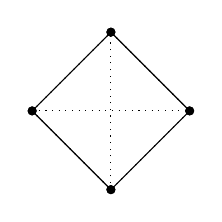
\begin{tikzpicture}[baseline=(current bounding box.center)]
  \pic at (0,0) {chamber4};
\draw (0,1) -- (1,0) -- (2,1) -- (1,2) -- (0,1);
\draw[fill] (0,1) circle [radius=0.05];
\draw[fill] (1,0) circle [radius=0.05];
\draw[fill] (2,1) circle [radius=0.05];
\draw[fill] (1,2) circle [radius=0.05];
\end{tikzpicture}
 &
$\begin{bmatrix}
1 & 0 & 1 \\
0 & 2 & 0 \\
0 & 1 & 0 \end{bmatrix}$
& $x@m = j = jd = da = \Box_{1,1}$
\\ \hline
\begin{tikzpicture}[baseline=(current bounding box.center)]
  \pic at (0,0) {chamber1};
\draw (0.85,0) -- (0.85,1.5);
\draw[fill] (0.85, 1.5) circle [radius=0.05];
\end{tikzpicture} &
$\begin{bmatrix}
0 & 0 & 1 & -1 & 3/2 \\
0 & 0 & 0 & 0 & 1/2 \\
1 & 1 & 0 & 0 & 0 \end{bmatrix}$ &
ABC, BAC &
$d$
 &
$\begin{bmatrix}
0 & 0 & 1 \\
0 & 1 & 0 \\
1 & 0 & 0 \end{bmatrix}$
& $\$x@m = d$
\\ & &
CAB, CBA &
$S$
 &
$\begin{bmatrix}
1 & 0 & 0 \\
0 & 1 & 0 \\
0 & 0 & 1 \end{bmatrix}$
& $\$x@m = S$
\\ & &
ACB, BCA &
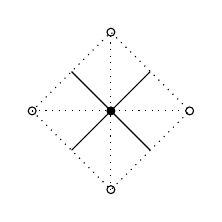
\begin{tikzpicture}[baseline=(current bounding box.center)]
  \pic at (0,0) {chamber4};
\draw (0.5,0.5) -- (1.5,1.5);
\draw (1.5,0.5) -- (0.5,1.5);
\draw[fill] (1,1) circle [radius=0.05];
\end{tikzpicture}
 &
$\begin{bmatrix}
0 & 1 & 0 \\
0 & 2 & 0 \\
1 & 0 & 1 \end{bmatrix}$
&  $x@m = a = dj$
\end{tabular}
\end{table}

\begin{table}
\caption{$o$-cohort of operators on polyhedra}
\begin{tabular}[t]{ c c|p{1cm} c c p{2cm} }
\hline \hline
$x \in \mathcal{W}$ & $M_{x}$ & $@$ & $\$x@m \in \mathcal{P}$ & $M_{\$x@m}$
& Note
\\ \hline
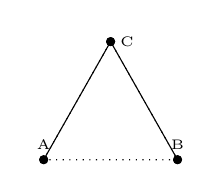
\begin{tikzpicture}[baseline=(current bounding box.center)]
  \pic at (0,0) {chamber1};
  \draw (0, 0) -- (0.85,1.5) -- (1.7, 0) ;
  \draw[fill] (0, 0) circle [radius=0.05] ;
  \draw[fill] (0.85, 1.5) circle [radius=0.05] ;
  \draw[fill] (1.7, 0) circle [radius=0.05] ;
\end{tikzpicture} &
$\begin{bmatrix}
1 & 0 & 0 \\
0 & 0 & 1 \\
0 & -1 & 2 \end{bmatrix}$ &
ABC, BAC &
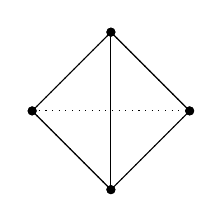
\begin{tikzpicture}[baseline=(current bounding box.center)]
  \pic at (0,0) {chamber4};
  \draw (1,0) -- (0,1) -- (1,2) -- (2,1) -- (1,0);
  \draw (1,0) -- (1,2);
  \draw[fill] (0,1) circle [radius=0.05];
  \draw[fill] (2,1) circle [radius=0.05];
  \draw[fill] (1,0) circle [radius=0.05];
  \draw[fill] (1,2) circle [radius=0.05];
\end{tikzpicture}
 &
 $\begin{bmatrix}
 1 & 0 & 1 \\
 0 & 3 & 0 \\
 0 & 2 & 0 \end{bmatrix}$
&  $\$x@m = n = kd = \Delta_{1,1}$
\\ & & ACB, BCA &
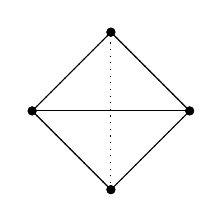
\begin{tikzpicture}[baseline=(current bounding box.center)]
  \pic at (0,0) {chamber4};
\draw (1,0) -- (0,1) -- (1,2) -- (2,1) -- (1,0);
\draw (0,1) -- (2,1);
\draw[fill] (0,1) circle [radius=0.05];
\draw[fill] (2,1) circle [radius=0.05];
\draw[fill] (1,0) circle [radius=0.05];
\draw[fill] (1,2) circle [radius=0.05];
\end{tikzpicture}
 &
 $\begin{bmatrix}
 1 & 0 & 1 \\
 0 & 3 & 0 \\
 0 & 2 & 0 \end{bmatrix}$
& $\$x@m = k = nd$
\\ & & CAB, CBA &
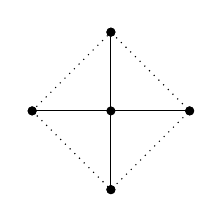
\begin{tikzpicture}[baseline=(current bounding box.center)]
  \pic at (0,0) {chamber4};
\draw (0,1) -- (2,1);
\draw (1,0) -- (1,2);
\draw[fill] (1,1) circle [radius=0.05];
\draw[fill] (0,1) circle [radius=0.05];
\draw[fill] (2,1) circle [radius=0.05];
\draw[fill] (1,0) circle [radius=0.05];
\draw[fill] (1,2) circle [radius=0.05];
\end{tikzpicture}
 &
$\begin{bmatrix}
1 & 1 & 1 \\
0 & 4 & 0 \\
0 & 2 & 0 \end{bmatrix}$
& $x@m = o = j^2 = \Box_{2,0}$
\\ \hline
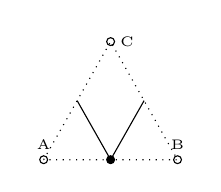
\begin{tikzpicture}[baseline=(current bounding box.center)]
  \pic at (0,0) {chamber1};
  \draw (0.425, 0.75) -- (0.85,0) -- (1.275, 0.75) ;
  \draw[fill] (0.85,0) circle [radius=0.05];
\end{tikzpicture} &
$\begin{bmatrix}
0 & -1 & 2 \\
0 & 0 & 1 \\
1 & 0 & 0 \end{bmatrix}$ &
ACB, BCA &
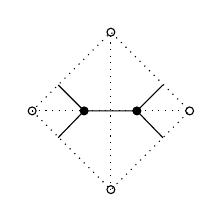
\begin{tikzpicture}[baseline=(current bounding box.center)]
  \pic at (0,0) {chamber4};
  \draw (0.33, 0.66) -- (0.66,1) -- (1.33,1) -- (1.66,1.33);
  \draw (0.33, 1.33) -- (0.66,1);
  \draw (1.33,1) -- (1.66,0.66);
  \draw[fill] (0.66,1) circle [radius=0.05];
  \draw[fill] (1.33,1) circle [radius=0.05];
\end{tikzpicture}
 &
 $\begin{bmatrix}
 0 & 2 & 0 \\
 0 & 3 & 0 \\
 1 & 0 & 1 \end{bmatrix}$
&  $\$x@m = t = zd$
\\ & & ABC, BAC &
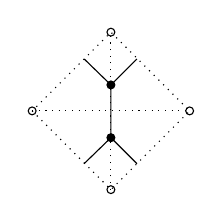
\begin{tikzpicture}[baseline=(current bounding box.center)]
  \pic at (0,0) {chamber4};
  \draw (0.66, 0.33) -- (1,0.66) -- (1,1.33) -- (1.33,1.66);
  \draw (1.33, 0.33) -- (1,0.66);
  \draw (1,1.33) -- (0.66,1.66);
  \draw[fill] (1,0.66) circle [radius=0.05];
  \draw[fill] (1,1.33) circle [radius=0.05];
\end{tikzpicture}
 &
 $\begin{bmatrix}
 0 & 2 & 0 \\
 0 & 3 & 0 \\
 1 & 0 & 1 \end{bmatrix}$
& $\$x@m = z = td$
\\ & & CAB, CBA &
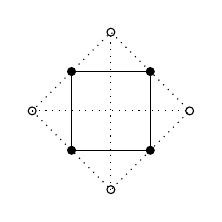
\begin{tikzpicture}[baseline=(current bounding box.center)]
  \pic at (0,0) {chamber4};
\draw (0.5,0.5) -- (1.5,0.5) -- (1.5,1.5) -- (0.5,1.5) -- (0.5,0.5);
\draw[fill] (0.5,0.5) circle [radius=0.05];
\draw[fill] (1.5,0.5) circle [radius=0.05];
\draw[fill] (1.5,1.5) circle [radius=0.05];
\draw[fill] (0.5,1.5) circle [radius=0.05];
\end{tikzpicture}
 &
$\begin{bmatrix}
0 & 2 & 0 \\
0 & 4 & 0 \\
1 & 1 & 1 \end{bmatrix}$
& $x@m = e = a^2$
\end{tabular}
\end{table}

\begin{table}
\caption{$u$-cohort of operators on polyhedra}
\begin{tabular}[t]{ c c|p{1cm} c c p{2cm} }
\hline \hline
$x \in \mathcal{W}$ & $M_{x}$ & $@$ & $\$x@m \in \mathcal{P}$ & $M_{\$x@m}$
& Note
\\ \hline
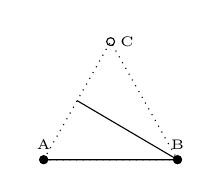
\begin{tikzpicture}[baseline=(current bounding box.center)]
  \pic at (0,0) {chamber1};
  \draw (0.425,0.75) -- (1.7, 0)  -- (0, 0);
  \draw[fill] (0, 0) circle [radius=0.05];
  \draw[fill] (1.7, 0) circle [radius=0.05];
\end{tikzpicture} &
$\begin{bmatrix}
1 & 1 & 0 & 0 & 0 \\
0 & 0 & 0 & 0 & 1 \\
0 & 0 & 1 & -1 & 2 \end{bmatrix}$ &
ABC &
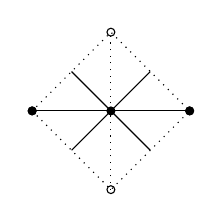
\begin{tikzpicture}[baseline=(current bounding box.center)]
  \pic at (0,0) {chamber4};
\draw (0,1) -- (2,1);
\draw (0.5,0.5) -- (1.5,1.5);
\draw (1.5,0.5) -- (0.5,1.5);

\draw[fill] (0,1) circle [radius=0.05];
\draw[fill] (1,1) circle [radius=0.05];
\draw[fill] (2,1) circle [radius=0.05];

\end{tikzpicture}
 &
$\begin{bmatrix}
1 & 1 & 0 \\
0 & 4 & 0 \\
0 & 2 & 1 \end{bmatrix}$
& $x@m = u = dcd = \Delta_{2,0}$
\\ & & ACB & $n$ &
$\begin{bmatrix}
1 & 0 & 1 \\
0 & 3 & 0 \\
0 & 2 & 0 \end{bmatrix}$
& $\$x@m = n$
\\ & & BAC & $S$ &
$\begin{bmatrix}
1 & 0 & 0 \\
0 & 1 & 0 \\
0 & 0 & 1 \end{bmatrix}$
& $\$x@m = S$
\\ \hline
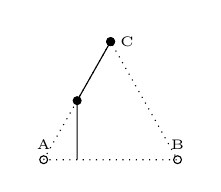
\begin{tikzpicture}[baseline=(current bounding box.center)]
  \pic at (0,0) {chamber1};
  \draw (0.85, 1.5) -- (0.425, 0.75)  -- (0.425, 0);
  \draw[fill] (0.85, 1.5) circle [radius=0.05];
  \draw[fill] (0.425, 0.75) circle [radius=0.05];
\end{tikzpicture} &
$\begin{bmatrix}
0 & 0 & 1 & -1 & 2 \\
0 & 0 & 0 & 0 & 1 \\
1 & 1 & 0 & 0 & 0 \end{bmatrix}$ &
 ACB & $t$ &
$\begin{bmatrix}
0 & 2 & 0 \\
0 & 3 & 0 \\
1 & 0 & 1 \end{bmatrix}$
& $\$x@m = t$
\\ & & CAB & $S$ &
$\begin{bmatrix}
1 & 0 & 0 \\
0 & 1 & 0 \\
0 & 0 & 1 \end{bmatrix}$
& $\$x@m = S$
\\ & &
CBA &
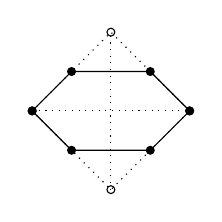
\begin{tikzpicture}[baseline=(current bounding box.center)]
  \pic at (0,0) {chamber4};
\draw (0,1) -- (0.5,0.5) -- (1.5,0.5) -- (2,1) -- (1.5,1.5) -- (0.5,1.5)
  -- (0,1);
\draw[fill] (0.5,0.5) circle [radius=0.05];
\draw[fill] (1.5,1.5) circle [radius=0.05];
\draw[fill] (1.5,0.5) circle [radius=0.05];
\draw[fill] (0.5,1.5) circle [radius=0.05];
\draw[fill] (0,1) circle [radius=0.05];
\draw[fill] (2,1) circle [radius=0.05];
\end{tikzpicture}
 &
$\begin{bmatrix}
1 & 2 & 0 \\
0 & 4 & 0 \\
0 & 1 & 1 \end{bmatrix}$
& $x@m = c$
\end{tabular}
\end{table}

\begin{table}%verify that the orientation is the same as in wythoff
\caption{$p$-cohort of operators on polyhedra}
\begin{tabular}[t]{ c c|p{1cm} c c p{2cm} }
\hline \hline
$x \in \mathcal{W}$ & $M_{x}$ & $@$ & $\$x@m \in \mathcal{P}$ & $M_{\$x@m}$
& Note
\\ \hline
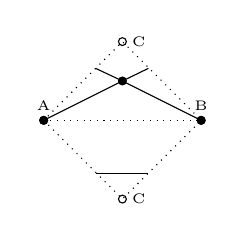
\begin{tikzpicture}[baseline=(current bounding box.center)]
  \pic at (0,0) {chamber2};
  \draw[fill] (1,1.5) circle [radius=0.05];
  \draw[fill] (0,1) circle [radius=0.05];
  \draw[fill] (2,1) circle [radius=0.05];
  \draw (2,1) -- (1,1.5) -- (0,1);
  \draw (0.66,1.66) -- (1,1.5) -- (1.33,1.66);
  \draw (0.66,0.33) -- (1.33,0.33);

\end{tikzpicture} &
$\begin{bmatrix}
1 & 1 & 0 & 0 & 1/2 \\
0 & 0 & 0 & 0 & 3/2 \\
0 & 0 & 1 & -1 & 2 \end{bmatrix}$ &
BAC &
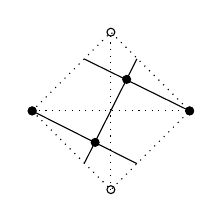
\begin{tikzpicture}[baseline=(current bounding box.center)]
  \pic at (0,0) {chamber4};
\draw (0,1) -- (1.33,0.33);
\draw (2,1) -- (0.66,1.66);
\draw (0.66,0.33) -- (1.33,1.66);
\draw[fill] (1.2,1.4) circle [radius=0.05];
\draw[fill] (0.8,0.6) circle [radius=0.05];
\draw[fill] (0,1) circle [radius=0.05];
\draw[fill] (2,1) circle [radius=0.05];

\end{tikzpicture}
 &
$\begin{bmatrix}
1 & 2 & 0 \\
0 & 5 & 0 \\
0 & 2 & 1 \end{bmatrix}$
&  $\$x@m = p = dpd = \Box_{2,1}$
\\ & & ACB &
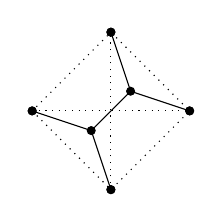
\begin{tikzpicture}[baseline=(current bounding box.center)]
  \pic at (0,0) {chamber4};
\draw (2,1) -- (1.25,1.25) -- (1,2);
\draw (0,1) -- (0.75,0.75) -- (1,0);
\draw (1.25,1.25) -- (0.75,0.75);

\draw[fill] (1,0) circle [radius=0.05];
\draw[fill] (1,2) circle [radius=0.05];
\draw[fill] (0,1) circle [radius=0.05];
\draw[fill] (2,1) circle [radius=0.05];
\draw[fill] (1.25,1.25) circle [radius=0.05];
\draw[fill] (0.75,0.75) circle [radius=0.05];

\end{tikzpicture}
 &
$\begin{bmatrix}
1 & 2 & 1 \\
0 & 5 & 0 \\
0 & 2 & 0 \end{bmatrix}$
& $\$x@m = rgr$
\\ \hline
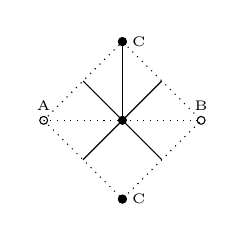
\begin{tikzpicture}[baseline=(current bounding box.center)]
  \pic at (0,0) {chamber2};
  \draw[fill] (1,0) circle [radius=0.05];
  \draw[fill] (1,1) circle [radius=0.05];
  \draw[fill] (1,2) circle [radius=0.05];
  \draw (0.5,0.5) -- (1.5,1.5);
  \draw (1.5,0.5) -- (0.5,1.5);
  \draw (1,1) -- (1,2);
\end{tikzpicture} &
$\begin{bmatrix}
0 & 0 & 1 & -1 & 2 \\
0 & 0 & 0 & 0 & 3/2 \\
1 & 1 & 0 & 0 & 1/2 \end{bmatrix}$ &
ACB &
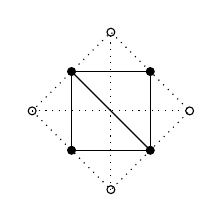
\begin{tikzpicture}[baseline=(current bounding box.center)]
  \pic at (0,0) {chamber4};
\draw (0.5,1.5) -- (1.5,1.5) -- (1.5,0.5) -- (0.5,0.5) -- (0.5,1.5);
\draw (1.5,0.5) -- (0.5,1.5);
\draw[fill] (0.5,1.5) circle [radius=0.05];
\draw[fill] (1.5,1.5) circle [radius=0.05];
\draw[fill] (1.5,0.5) circle [radius=0.05];
\draw[fill] (0.5,0.5) circle [radius=0.05];
\end{tikzpicture}
 &
$\begin{bmatrix}
0 & 2 & 0 \\
0 & 5 & 0 \\
1 & 2 & 1 \end{bmatrix}$
& $\$x@m = rsr$
\\ & & BCA &
$p$
 &
$\begin{bmatrix}
1 & 2 & 0 \\
0 & 5 & 0 \\
0 & 2 & 1 \end{bmatrix}$
&  $\$x@m = p$
\end{tabular}
\end{table}

\begin{table}
\caption{$g$-cohort of operators on polyhedra}
\begin{tabular}[t]{ c c|p{1cm} c c p{2cm} }
\hline \hline
$x \in \mathcal{W}$ & $M_{x}$ & $@$ & $\$x@m \in \mathcal{P}$ & $M_{\$x@m}$
& Note
\\ \hline
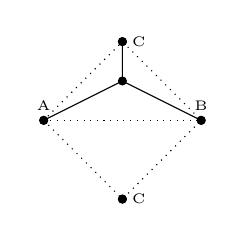
\begin{tikzpicture}[baseline=(current bounding box.center)]
  \pic at (0,0) {chamber2};
  \draw[fill] (1,1.5) circle [radius=0.05];
  \draw[fill] (1,0) circle [radius=0.05];
  \draw[fill] (1,2) circle [radius=0.05];
  \draw[fill] (0,1) circle [radius=0.05];
  \draw[fill] (2,1) circle [radius=0.05];
  \draw (1,2) -- (1,1.5) -- (0,1);
  \draw (1,1.5) -- (2,1);
\end{tikzpicture} &
$\begin{bmatrix}
1 & -1 & 2 \\
0 & 0 & 3/2 \\
0 & 0 & 1/2 \end{bmatrix}$ &
ABC BCA CAB (CBA) (BAC) (ACB)&
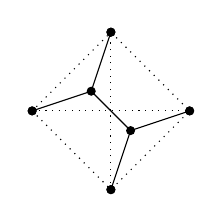
\begin{tikzpicture}[baseline=(current bounding box.center)]
  \pic at (0,0) {chamber4};
\draw (0,1) -- (0.75,1.25) -- (1,2);
\draw (2,1) -- (1.25,0.75) -- (1,0);
\draw (0.75,1.25) -- (1.25,0.75);

\draw[fill] (1,0) circle [radius=0.05];
\draw[fill] (1,2) circle [radius=0.05];
\draw[fill] (0,1) circle [radius=0.05];
\draw[fill] (2,1) circle [radius=0.05];
\draw[fill] (0.75,1.25) circle [radius=0.05];
\draw[fill] (1.25,0.75) circle [radius=0.05];

\end{tikzpicture}
 &
$\begin{bmatrix}
1 & 2 & 1 \\
0 & 5 & 0 \\
0 & 2 & 0 \end{bmatrix}$
& $\$x@m = g$
\\
\hline
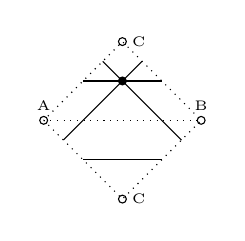
\begin{tikzpicture}[baseline=(current bounding box.center)]
  \pic at (0,0) {chamber2};
  \draw[fill] (1,1.5) circle [radius=0.05];
  \draw (0.5,1.5) -- (1.5,1.5);
  \draw (0.5,0.5) -- (1.5,0.5);
  \draw (0.75,1.75) -- (1.75,0.75);
  \draw (1.25,1.75) -- (0.25,0.75);

\end{tikzpicture} &
$\begin{bmatrix}
0 & 0 & 1/2 \\
0 & 0 & 3/2 \\
1 & -1 & 2 \end{bmatrix}$ &
ABC BCA CAB (CBA) (BAC) (ACB)&
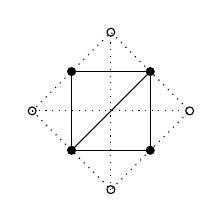
\begin{tikzpicture}[baseline=(current bounding box.center)]
  \pic at (0,0) {chamber4};
\draw (0.5,1.5) -- (1.5,1.5) -- (1.5,0.5) -- (0.5,0.5) -- (0.5,1.5);
\draw (1.5,1.5) -- (0.5,0.5);
\draw[fill] (0.5,1.5) circle [radius=0.05];
\draw[fill] (1.5,1.5) circle [radius=0.05];
\draw[fill] (1.5,0.5) circle [radius=0.05];
\draw[fill] (0.5,0.5) circle [radius=0.05];
\end{tikzpicture}
 &
$\begin{bmatrix}
0 & 2 & 0 \\
0 & 5 & 0 \\
1 & 2 & 1 \end{bmatrix}$
& $\$x@m = s$
\end{tabular}
\end{table}


\begin{table}
\caption{$l$-cohort of operators on polyhedra}
\begin{tabular}[t]{ c c|p{1cm} c c p{2cm} }
\hline \hline
$x \in \mathcal{W}$ & $M_{x}$ & $@$ & $\$x@m \in \mathcal{P}$ & $M_{\$x@m}$
& Note
\\ \hline
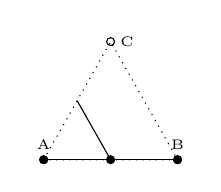
\begin{tikzpicture}[baseline=(current bounding box.center)]
  \pic at (0,0) {chamber1};
\draw[fill] (0, 0) circle [radius=0.05];
\draw[fill] (1.7, 0) circle [radius=0.05];
\draw[fill] (0.85, 0) circle [radius=0.05];
\draw (0, 0) -- (1.7, 0) ;
\draw (0.425, 0.75) -- (0.85, 0) ;
\end{tikzpicture} &
$\begin{bmatrix}
1 & 1 & 0 & 0 & 1/2 \\
0 & 0 & 0 & 0 & 2 \\
0 & 0 & 1 & -1 & ? \end{bmatrix}$ &
ABC&
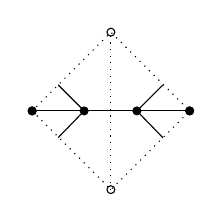
\begin{tikzpicture}[baseline=(current bounding box.center)]
  \pic at (0,0) {chamber4};
\draw (2,1) -- (0,1) ;
\draw (0.33,0.66) -- (0.66,1) -- (0.33,1.33);
\draw (1.66,0.66) -- (1.33,1) -- (1.66,1.33);
\draw[fill] (0,1) circle [radius=0.05];
\draw[fill] (0.66,1) circle [radius=0.05];
\draw[fill] (1.33,1) circle [radius=0.05];
\draw[fill] (2,1) circle [radius=0.05];
\end{tikzpicture}
 &
$\begin{bmatrix}
1 & 2 & 0 \\
0 & 5 & 0 \\
0 & 2 & 1 \end{bmatrix}$
& $\$x@m = dld$
\\ & & BAC& $S$ &
$\begin{bmatrix}
1 & 0 & 0 \\
0 & 1 & 0 \\
0 & 0 & 1 \end{bmatrix}$
& $\$x@m = S$
\\ & & BCA&
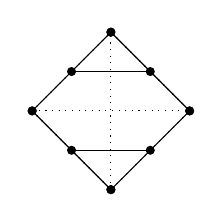
\begin{tikzpicture}[baseline=(current bounding box.center)]
  \pic at (0,0) {chamber4};
\draw (0,1) -- (1,2) -- (2,1) -- (1,0) -- (0,1);
\draw (0.5, 1.5) -- (1.5,1.5);
\draw (0.5, 0.5) -- (1.5,0.5);
\draw[fill] (0,1) circle [radius=0.05];
\draw[fill] (2,1) circle [radius=0.05];
\draw[fill] (1,0) circle [radius=0.05];
\draw[fill] (1,2) circle [radius=0.05];
\draw[fill] (0.5,0.5) circle [radius=0.05];
\draw[fill] (1.5,1.5) circle [radius=0.05];
\draw[fill] (1.5,0.5) circle [radius=0.05];
\draw[fill] (0.5,1.5) circle [radius=0.05];
\end{tikzpicture}
 &
$\begin{bmatrix}
1 & 2 & 1 \\
0 & 6 & 0 \\
0 & 3 & 0 \end{bmatrix}$
& $x@m$
\\ \hline
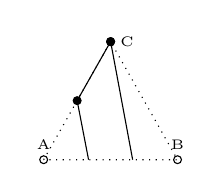
\begin{tikzpicture}[baseline=(current bounding box.center)]
  \pic at (0,0) {chamber1};
\draw[fill] (0.85, 1.5) circle [radius=0.05];
\draw[fill] (0.425, 0.75) circle [radius=0.05];
\draw (0.57, 0) -- (0.425, 0.75) -- (0.85, 1.5) -- (1.13, 0);
\end{tikzpicture} &
$\begin{bmatrix}
1 & 1 & 0 & 0 & 1/2 \\
0 & 0 & 0 & 0 & 2 \\
0 & 0 & 1 & -1 & ? \end{bmatrix}$ &
CBA&
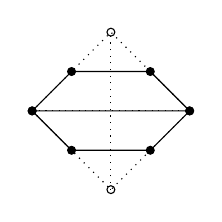
\begin{tikzpicture}[baseline=(current bounding box.center)]
  \pic at (0,0) {chamber4};
\draw (0,1) -- (2,1) -- (1.5,0.5) -- (0.5,0.5) --
      (0,1) -- (0.5,1.5) -- (1.5,1.5) -- (2,1);
\draw[fill] (0,1) circle [radius=0.05];
\draw[fill] (0.5,0.5) circle [radius=0.05];
\draw[fill] (1.5,1.5) circle [radius=0.05];
\draw[fill] (1.5,0.5) circle [radius=0.05];
\draw[fill] (0.5,1.5) circle [radius=0.05];
\draw[fill] (2,1) circle [radius=0.05];
\end{tikzpicture}
 &
$\begin{bmatrix}
1 & 2 & 0 \\
0 & 5 & 0 \\
0 & 2 & 1 \end{bmatrix}$
& $\$x@m = l$
\\ & & CAB& $S$ &
$\begin{bmatrix}
1 & 0 & 0 \\
0 & 1 & 0 \\
0 & 0 & 1 \end{bmatrix}$
& $\$x@m = S$
\\ & & ACB&
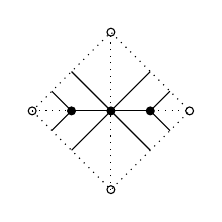
\begin{tikzpicture}[baseline=(current bounding box.center)]
  \pic at (0,0) {chamber4};
\draw (0.5, 1) -- (1.5,1);
\draw (0.5, 0.5) -- (1.5,1.5);
\draw (0.5, 1.5) -- (1.5,0.5);
\draw (0.25, 1.25) -- (0.5, 1) -- (0.25, 0.75);
\draw (1.75, 1.25) -- (1.5, 1) -- (1.75, 0.75);
\draw[fill] (0.5,1) circle [radius=0.05];
\draw[fill] (1,1) circle [radius=0.05];
\draw[fill] (1.5,1) circle [radius=0.05];
\end{tikzpicture}
 &
$\begin{bmatrix}
0 & 3 & 0 \\
0 & 6 & 0 \\
1 & 2 & 1 \end{bmatrix}$
& $x@m$
\end{tabular}
\end{table}

\begin{table}
\caption{$L_0$-cohort of operators on polyhedra}
\begin{tabular}[t]{ c c|p{1cm} c c p{2cm} }
\hline \hline
$x \in \mathcal{W}$ & $M_{x}$ & $@$ & $\$x@m \in \mathcal{P}$ & $M_{\$x@m}$
& Note
\\ \hline
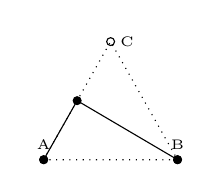
\begin{tikzpicture}[baseline=(current bounding box.center)]
  \pic at (0,0) {chamber1};
\draw[fill] (0, 0) circle [radius=0.05];
\draw[fill] (0.425, 0.75) circle [radius=0.05];
\draw[fill] (1.7, 0) circle [radius=0.05];
\draw (0,0) -- (0.425, 0.75) -- (1.7, 0);
\end{tikzpicture} &
$\begin{bmatrix}
1 & 1 & 0 & 0 & 1/2 \\
0 & 0 & 0 & 0 & 2 \\
0 & 0 & 1 & -1 & ? \end{bmatrix}$ &
ABC&
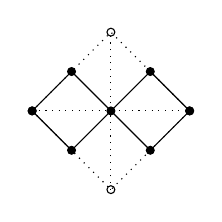
\begin{tikzpicture}[baseline=(current bounding box.center)]
  \pic at (0,0) {chamber4};
\draw (0,1) -- (0.5,0.5) -- (1.5,1.5) --
      (2,1) -- (1.5,0.5) -- (0.5,1.5) -- (0,1);
\draw[fill] (0,1) circle [radius=0.05];
\draw[fill] (1,1) circle [radius=0.05];
\draw[fill] (2,1) circle [radius=0.05];
\draw[fill] (0.5,0.5) circle [radius=0.05];
\draw[fill] (0.5,1.5) circle [radius=0.05];
\draw[fill] (1.5,1.5) circle [radius=0.05];
\draw[fill] (1.5,0.5) circle [radius=0.05];
\end{tikzpicture}
 &
$\begin{bmatrix}
1 & 3 & 0 \\
0 & 6 & 0 \\
0 & 2 & 1 \end{bmatrix}$
&$x@m = dL_0d$
\\ & & BAC &
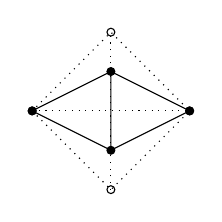
\begin{tikzpicture}[baseline=(current bounding box.center)]
  \pic at (0,0) {chamber4};
\draw (1,1.5) -- (0,1) -- (1,0.5) -- (1,1.5) -- (2,1) -- (1,0.5);
\draw[fill] (0,1) circle [radius=0.05];
\draw[fill] (1,0.5) circle [radius=0.05];
\draw[fill] (1,1.5) circle [radius=0.05];
\draw[fill] (2,1) circle [radius=0.05];
\end{tikzpicture}
 &
$\begin{bmatrix}
1 & 2 & 0 \\
0 & 5 & 0 \\
0 & 2 & 1 \end{bmatrix}$
& $\$x@m =$ Lozenge \dag
\\ & & BCA &
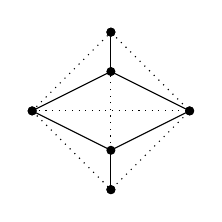
\begin{tikzpicture}[baseline=(current bounding box.center)]
  \pic at (0,0) {chamber4};
\draw (0,1) -- (1,0.5) -- (2,1) -- (1,1.5) -- (0,1);
\draw (1,0) -- (1,0.5);
\draw (1,2) -- (1,1.5);
\draw[fill] (0,1) circle [radius=0.05];
\draw[fill] (1,0) circle [radius=0.05];
\draw[fill] (1,2) circle [radius=0.05];
\draw[fill] (1,0.5) circle [radius=0.05];
\draw[fill] (1,1.5) circle [radius=0.05];
\draw[fill] (2,1) circle [radius=0.05];
\end{tikzpicture}
 &
$\begin{bmatrix}
1 & 2 & 1 \\
0 & 6 & 0 \\
0 & 3 & 0 \end{bmatrix}$
& $x@m = jk$
\\ \hline
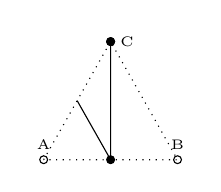
\begin{tikzpicture}[baseline=(current bounding box.center)]
  \pic at (0,0) {chamber1};
\draw (0.85,1.5) -- (0.85,0) -- (0.425, 0.75);
\draw[fill] (0.85, 1.5) circle [radius=0.05];
\draw[fill] (0.85, 0) circle [radius=0.05];
\end{tikzpicture} &
$\begin{bmatrix}
0 & 0 & 1 & -1 & 3/2 \\
0 & 0 & 0 & 0 & 1/2 \\
1 & 1 & 0 & 0 & 0 \end{bmatrix}$ &
CAB &
Lozenge
 &
$\begin{bmatrix}
1 & 2 & 0 \\
0 & 5 & 0 \\
0 & 2 & 1 \end{bmatrix}$
& $\$x@m =$ Lozenge \dag
\\ & & CBA &
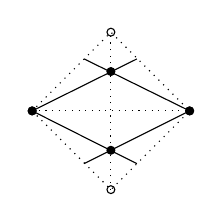
\begin{tikzpicture}[baseline=(current bounding box.center)]
  \pic at (0,0) {chamber4};
\draw (1.33,1.66) -- (0,1) -- (1.33,0.33);
\draw (0.66,1.66) -- (2,1) -- (0.66,0.33);

\draw[fill] (0,1) circle [radius=0.05];
\draw[fill] (1,0.5) circle [radius=0.05];
\draw[fill] (1,1.5) circle [radius=0.05];
\draw[fill] (2,1) circle [radius=0.05];
\end{tikzpicture}
 &
$\begin{bmatrix}
1 & 2 & 0 \\
0 & 6 & 0 \\
0 & 3 & 1 \end{bmatrix}$
& $x@m = L_0$
\\ & & BCA &
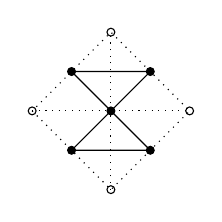
\begin{tikzpicture}[baseline=(current bounding box.center)]
  \pic at (0,0) {chamber4};
\draw (0.5,0.5) -- (1.5,0.5) --
      (0.5,1.5) -- (1.5,1.5) -- (0.5,0.5);
\draw[fill] (1,1) circle [radius=0.05];
\draw[fill] (0.5,0.5) circle [radius=0.05];
\draw[fill] (0.5,1.5) circle [radius=0.05];
\draw[fill] (1.5,1.5) circle [radius=0.05];
\draw[fill] (1.5,0.5) circle [radius=0.05];
\end{tikzpicture}
 &
$\begin{bmatrix}
0 & 3 & 0 \\
0 & 6 & 0 \\
1 & 2 & 1 \end{bmatrix}$
&$x@m = djk$
\end{tabular}
\end{table}

\begin{table}
\caption{$q$-cohort of operators on polyhedra}
\begin{tabular}[t]{ c c|p{1cm} c c p{2cm} }
\hline \hline
$x \in \mathcal{W}$ & $M_{x}$ & $@$ & $\$x@m \in \mathcal{P}$ & $M_{\$x@m}$
& Note
\\ \hline
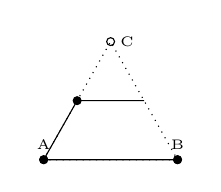
\begin{tikzpicture}[baseline=(current bounding box.center)]
  \pic at (0,0) {chamber1};
\draw[fill] (0, 0) circle [radius=0.05];
\draw[fill] (0.425, 0.75) circle [radius=0.05];
\draw[fill] (1.7, 0) circle [radius=0.05];
\draw (1.7,0) -- (0, 0) -- (0.425, 0.75) -- (1.275, 0.75) ;
\end{tikzpicture} &
$\begin{bmatrix}
1 & 1 & 0 & 0 & 1/2 \\
0 & 0 & 0 & 0 & 2 \\
0 & 0 & 1 & -1 & ? \end{bmatrix}$ &
ABC&
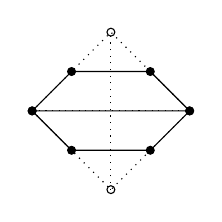
\begin{tikzpicture}[baseline=(current bounding box.center)]
  \pic at (0,0) {chamber4};
\draw (0,1) -- (2,1) -- (1.5,0.5) -- (0.5,0.5) --
      (0,1) -- (0.5,1.5) -- (1.5,1.5) -- (2,1);
\draw[fill] (0,1) circle [radius=0.05];
\draw[fill] (0.5,0.5) circle [radius=0.05];
\draw[fill] (1.5,1.5) circle [radius=0.05];
\draw[fill] (1.5,0.5) circle [radius=0.05];
\draw[fill] (0.5,1.5) circle [radius=0.05];
\draw[fill] (2,1) circle [radius=0.05];
\end{tikzpicture}
 &
$\begin{bmatrix}
1 & 2 & 0 \\
0 & 5 & 0 \\
0 & 2 & 1 \end{bmatrix}$
& $\$x@m = l$
\\ & & BAC &
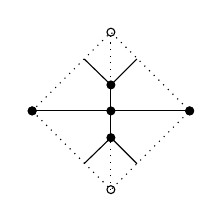
\begin{tikzpicture}[baseline=(current bounding box.center)]
  \pic at (0,0) {chamber4};
\draw (1,1.33) -- (1,0.66) ;
\draw (0,1) -- (2,1) ;
\draw (0.66,0.33) -- (1,0.66) -- (1.33,0.33);
\draw (0.66,1.66) -- (1,1.33) -- (1.33,1.66);
\draw[fill] (0,1) circle [radius=0.05];
\draw[fill] (1,1) circle [radius=0.05];
\draw[fill] (1,0.66) circle [radius=0.05];
\draw[fill] (1,1.33) circle [radius=0.05];
\draw[fill] (2,1) circle [radius=0.05];
\end{tikzpicture}
 &
$\begin{bmatrix}
1 & 3 & 0 \\
0 & 6 & 0 \\
0 & 2 & 1 \end{bmatrix}$
& $x@m = q$
\\ & & ACB & $k$&
$\begin{bmatrix}
1 & 0 & 1 \\
0 & 3 & 0 \\
0 & 2 & 0 \end{bmatrix}$
& $\$x@m = k$
\\ \hline
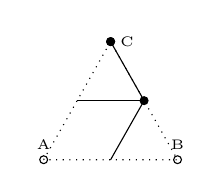
\begin{tikzpicture}[baseline=(current bounding box.center)]
  \pic at (0,0) {chamber1};
\draw (0.85,1.5) -- (1.275, 0.75) -- (0.85, 0);
\draw (1.275, 0.75) -- (0.425, 0.75);
\draw[fill] (0.85, 1.5) circle [radius=0.05];
\draw[fill] (1.275, 0.75) circle [radius=0.05];
\end{tikzpicture} &
$\begin{bmatrix}
0 & 0 & 1 & -1 & 3/2 \\
0 & 0 & 0 & 0 & 1/2 \\
1 & 1 & 0 & 0 & 0 \end{bmatrix}$ &
CBA &
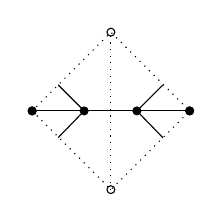
\begin{tikzpicture}[baseline=(current bounding box.center)]
  \pic at (0,0) {chamber4};
\draw (2,1) -- (0,1) ;
\draw (0.33,0.66) -- (0.66,1) -- (0.33,1.33);
\draw (1.66,0.66) -- (1.33,1) -- (1.66,1.33);
\draw[fill] (0,1) circle [radius=0.05];
\draw[fill] (0.66,1) circle [radius=0.05];
\draw[fill] (1.33,1) circle [radius=0.05];
\draw[fill] (2,1) circle [radius=0.05];
\end{tikzpicture}
 &
$\begin{bmatrix}
1 & 2 & 0 \\
0 & 5 & 0 \\
0 & 2 & 1 \end{bmatrix}$
& $\$x@m = dld$
\\ & & CAB &
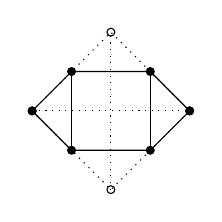
\begin{tikzpicture}[baseline=(current bounding box.center)]
  \pic at (0,0) {chamber4};
\draw (0,1) -- (0.5,0.5) -- (1.5,0.5) --
      (2,1) -- (1.5,1.5) -- (0.5,1.5) --  (0,1);
\draw (0.5,0.5) -- (0.5,1.5);
\draw (1.5,0.5) -- (1.5,1.5);

\draw[fill] (0,1) circle [radius=0.05];
\draw[fill] (0.5,0.5) circle [radius=0.05];
\draw[fill] (1.5,1.5) circle [radius=0.05];
\draw[fill] (1.5,0.5) circle [radius=0.05];
\draw[fill] (0.5,1.5) circle [radius=0.05];

\draw[fill] (2,1) circle [radius=0.05];
\end{tikzpicture}
 &
$\begin{bmatrix}
1 & 2 & 0 \\
0 & 6 & 0 \\
0 & 3 & 1 \end{bmatrix}$
& $x@m = dqd$
\\ & & BCA & $t$&
$\begin{bmatrix}
0 & 2 & 0 \\
0 & 3 & 0 \\
1 & 0 & 1 \end{bmatrix}$
& $\$x@m = t$
\end{tabular}
\end{table}

\begin{table}
\caption{$m$-cohort of operators on polyhedra}
\begin{tabular}[t]{ c c|p{1cm} c c p{2cm} }
\hline \hline
$x \in \mathcal{W}$ & $M_{x}$ & $@$ & $\$x@m \in \mathcal{P}$ & $M_{\$x@m}$
& Note
\\ \hline
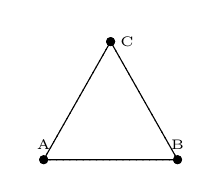
\begin{tikzpicture}[baseline=(current bounding box.center)]
  \pic at (0,0) {chamber1};
\draw (0, 0) -- (0.85,1.5) -- (1.7, 0) -- (0, 0) ;
\draw[fill] (0, 0) circle [radius=0.05];
\draw[fill] (0.85, 1.5) circle [radius=0.05];
\draw[fill] (1.7, 0) circle [radius=0.05];
\end{tikzpicture} &
$\begin{bmatrix}
1 & 0 & 0 \\
0 & 1 & 0 \\
0 & 0 & 1 \end{bmatrix}$ &
All &
\begin{tikzpicture}[baseline=(current bounding box.center)]
  \pic at (0,0) {chamber4};
\draw (0,1) -- (1,0) -- (2,1) -- (1,2) -- (0,1);
\draw (0,1) -- (2,1);
\draw (1,0) -- (1,2);
\draw[fill] (0,1) circle [radius=0.05];
\draw[fill] (1,0) circle [radius=0.05];
\draw[fill] (1,1) circle [radius=0.05];
\draw[fill] (2,1) circle [radius=0.05];
\draw[fill] (1,2) circle [radius=0.05];
\end{tikzpicture}
 &
$\begin{bmatrix}
1 & 1 & 1 \\
0 & 6 & 0 \\
0 & 4 & 0 \end{bmatrix}$
& $x = S$
$xm = m = kj$
\\ \hline
\begin{tikzpicture}[baseline=(current bounding box.center)]
  \pic at (0,0) {chamber1};
\draw (0.85, 0) -- (0.85,0.5);
\draw (0.425,0.75) -- (0.85,0.5) -- (1.275,0.75);
\draw[fill] (0.85, 0.5) circle [radius=0.05];
\end{tikzpicture} &
$\begin{bmatrix}
0 & 0 & 1 \\
0 & 1 & 0 \\
1 & 0 & 0 \end{bmatrix}$ &
All &
\begin{tikzpicture}[baseline=(current bounding box.center)]
  \pic at (0,0) {chamber4};
  \draw (0.75,1.25) -- (1.25,1.25) -- (1.25,0.75) -- (0.75,0.75) -- (0.75,1.25);
  \draw (0.75,1.25) -- (0.5,1.5);
  \draw (1.25,1.25) -- (1.5,1.5);
  \draw (1.25,0.75) -- (1.5,0.5);
  \draw (0.75,0.75) -- (0.5,0.5);
  \draw[fill] (0.75,1.25) circle [radius=0.05];
  \draw[fill] (1.25,1.25) circle [radius=0.05];
  \draw[fill] (1.25,0.75) circle [radius=0.05];
  \draw[fill] (0.75,0.75) circle [radius=0.05];
\end{tikzpicture}
 &
$\begin{bmatrix}
0 & 4 & 0 \\
0 & 6 & 0 \\
1 & 1 & 1 \end{bmatrix}$
& $x = d$
$xm = b = ta$
\end{tabular}
\end{table}

\begin{table}
\caption{$K$-cohort of operators on polyhedra}
\begin{tabular}[t]{ c c|p{1cm} c c p{2cm} }
\hline \hline
$x \in \mathcal{W}$ & $M_{x}$ & $@$ & $\$x@m \in \mathcal{P}$ & $M_{\$x@m}$
& Note
\\ \hline
\begin{tikzpicture}[baseline=(current bounding box.center)]
  \pic at (0,0) {chamber1};
\draw[fill] (0, 0) circle [radius=0.05];
\draw[fill] (0.85, 1.5) circle [radius=0.05];
\draw[fill] (1.7, 0) circle [radius=0.05];
\draw[fill] (0.85, 0) circle [radius=0.05];

\draw (0, 0) -- (0.85, 1.5) -- (0.85, 0) -- (1.7, 0) ;
\end{tikzpicture} &
$\begin{bmatrix}
1 & 0 & 1/2 \\
0 & 0 & 2 \\
0 & -1 & ? \end{bmatrix}$ &
ABC&
\begin{tikzpicture}[baseline=(current bounding box.center)]
  \pic at (0,0) {chamber4};
  \draw (0,1) -- (1,0) -- (2,1) -- (1,2) -- (0,1);
  \draw (0.66,1) -- (1,0) -- (1.33,1) -- (1,2) -- (0.66,1);
  \draw (0.66,1) -- (1.33,1);
  \draw[fill] (0,1) circle [radius=0.05];
  \draw[fill] (1,0) circle [radius=0.05];
  \draw[fill] (2,1) circle [radius=0.05];
  \draw[fill] (1,2) circle [radius=0.05];

  \draw[fill] (0.66,1) circle [radius=0.05];
  \draw[fill] (1.33,1) circle [radius=0.05];
\end{tikzpicture}
 &
$\begin{bmatrix}
1 & 2 & 1 \\
0 & 7 & 0 \\
0 & 4 & 0 \end{bmatrix}$
& $\$x@m$ \dag
\\ & & ACB &
\begin{tikzpicture}[baseline=(current bounding box.center)]
  \pic at (0,0) {chamber4};
  \draw (0,1) -- (2,1);
  \draw (1,0) -- (0.5,0.5) -- (1.5,1.5) --
        (1,2) -- (0.5,1.5) -- (1.5,0.5) -- (1,0);
  \draw[fill] (0,1) circle [radius=0.05];
  \draw[fill] (1,0) circle [radius=0.05];
  \draw[fill] (2,1) circle [radius=0.05];
  \draw[fill] (1,2) circle [radius=0.05];
  \draw[fill] (0.5,0.5) circle [radius=0.05];
  \draw[fill] (0.5,1.5) circle [radius=0.05];
  \draw[fill] (1.5,1.5) circle [radius=0.05];
  \draw[fill] (1.5,0.5) circle [radius=0.05];
\end{tikzpicture}
 &
$\begin{bmatrix}
1 & 3 & 1 \\
0 & 8 & 0 \\
0 & 4 & 0 \end{bmatrix}$
& $x@m$
\\ & & CAB &
\begin{tikzpicture}[baseline=(current bounding box.center)]
  \pic at (0,0) {chamber4};
  \draw (0,1) -- (2,1);
  \draw (0,1) -- (1,0.5) -- (2,1) -- (1,1.5) -- (0,1);
  \draw (1,0.5) -- (1,0);
  \draw (1,1.5) -- (1,2);
  \draw[fill] (0,1) circle [radius=0.05];
  \draw[fill] (1,0) circle [radius=0.05];
  \draw[fill] (2,1) circle [radius=0.05];
  \draw[fill] (1,2) circle [radius=0.05];
  \draw[fill] (1,1.5) circle [radius=0.05];
  \draw[fill] (1,0.5) circle [radius=0.05];
\end{tikzpicture}
 &
$\begin{bmatrix}
1 & 2 & 1 \\
0 & 7 & 0 \\
0 & 4 & 0 \end{bmatrix}$
& $\$x@m = K$
\\ \hline
\begin{tikzpicture}[baseline=(current bounding box.center)]
  \pic at (0,0) {chamber1};
\draw[fill] (0.425, 0) circle [radius=0.05];
\draw[fill] (1.275, 0.75) circle [radius=0.05];
\draw (0.425, 0.75) -- (0.425, 0) -- (1.275, 0.75) -- (1.275, 0) ;
\end{tikzpicture} &
$\begin{bmatrix}
1 & 0 & 1/2 \\
0 & 0 & 2 \\
0 & -1 & ? \end{bmatrix}$ &
ABC &
\begin{tikzpicture}[baseline=(current bounding box.center)]
  \pic at (0,0) {chamber4};
  \draw (0.5,1) -- (1,0.5) -- (1.5,1) -- (1,1.5) -- (0.5,1);
  \draw (1,0.5) -- (1,1.5);
  \draw (0.25,0.75) -- (0.5,1) -- (0.25,1.25);
  \draw (1.75,0.75) -- (1.5,1) -- (1.75,1.25);
  \draw[fill] (0.5,1) circle [radius=0.05];
  \draw[fill] (1,0.5) circle [radius=0.05];
  \draw[fill] (1.5,1) circle [radius=0.05];
  \draw[fill] (1,1.5) circle [radius=0.05];
\end{tikzpicture}
 &
$\begin{bmatrix}
1 & 2 & 1 \\
0 & 7 & 0 \\
0 & 4 & 0 \end{bmatrix}$
& $\$x@m$ \dag
\\ & & ACB&
\begin{tikzpicture}[baseline=(current bounding box.center)]
  \pic at (0,0) {chamber4};
  \draw (0.75,1.75) -- (1,1.5) -- (1.66,1.33) --
        (1.66,0.66) -- (1, 0.5) -- (0.75, 0.25);
  \draw (1.25,1.75) -- (1,1.5) -- (0.33,1.33) --
        (0.33,0.66) -- (1, 0.5) -- (1.25, 0.25);

  \draw[fill] (0.33,1.33) circle [radius=0.05];
  \draw[fill] (1.66,1.33) circle [radius=0.05];
  \draw[fill] (1.66,0.66) circle [radius=0.05];
  \draw[fill] (0.33,0.66) circle [radius=0.05];

  \draw[fill] (1,0.5) circle [radius=0.05];
  \draw[fill] (1,1.5) circle [radius=0.05];
\end{tikzpicture}
 &
$\begin{bmatrix}
0 & 4 & 0 \\
0 & 8 & 0 \\
1 & 3 & 1 \end{bmatrix}$
& $x@m$
\\ & & CAB&
\begin{tikzpicture}[baseline=(current bounding box.center)]
  \pic at (0,0) {chamber4};
  \draw (1,1.25) -- (0.5,1.5) -- (1.5,1.5) -- (1,1.25);
  \draw (1,0.75) -- (0.5,0.5) -- (1.5,0.5) -- (1,0.75);
  \draw (1,0.75) -- (1,1.25);
  \draw[fill] (0.5,1.5) circle [radius=0.05];
  \draw[fill] (1.5,1.5) circle [radius=0.05];
  \draw[fill] (1.5,0.5) circle [radius=0.05];
  \draw[fill] (0.5,0.5) circle [radius=0.05];

  \draw[fill] (1,0.75) circle [radius=0.05];
  \draw[fill] (1,1.25) circle [radius=0.05];
\end{tikzpicture}
 &
$\begin{bmatrix}
0 & 4 & 0 \\
0 & 7 & 0 \\
1 & 2 & 1 \end{bmatrix}$
& $\$x@m = dK$
\end{tabular}
\end{table}


\begin{table}
\caption{$M$-cohort of operators on polyhedra}
\begin{tabular}[t]{ c c|p{1cm} c c p{2cm} }
\hline \hline
$x \in \mathcal{W}$ & $M_{x}$ & $@$ & $\$x@m \in \mathcal{P}$ & $M_{\$x@m}$
& Note
\\ \hline
\begin{tikzpicture}[baseline=(current bounding box.center)]
  \pic at (0,0) {chamber1};
\draw[fill] (0, 0) circle [radius=0.05];
\draw[fill] (1.275, 0.75) circle [radius=0.05];
\draw[fill] (1.7, 0) circle [radius=0.05];
\draw (0, 0) -- (1.275, 0.75) -- (1.7, 0) ;
\draw (1.275, 0.75) -- (0.425, 0.75) ;

\end{tikzpicture} &
$\begin{bmatrix}
1 & 1 & 0 & 0 & 1/2 \\
0 & 0 & 0 & 0 & 2 \\
0 & 0 & 1 & -1 & ? \end{bmatrix}$ &
ABC&
\begin{tikzpicture}[baseline=(current bounding box.center)]
  \pic at (0,0) {chamber4};
\draw (1.33,1.66) -- (0,1) -- (1.33,0.33);
\draw (0.66,1.66) -- (2,1) -- (0.66,0.33);
\draw (1,0.5) -- (1,1.5);
\draw[fill] (0,1) circle [radius=0.05];
\draw[fill] (1,0.5) circle [radius=0.05];
\draw[fill] (1,1.5) circle [radius=0.05];
\draw[fill] (2,1) circle [radius=0.05];
\end{tikzpicture}
 &
$\begin{bmatrix}
1 & 2 & 0 \\
0 & 7 & 0 \\
0 & 4 & 1 \end{bmatrix}$
& $\$x@m = L_{-1}$
\\ & & BCA &
\begin{tikzpicture}[baseline=(current bounding box.center)]
  \pic at (0,0) {chamber4};
\draw (0,1) -- (2,1);
\draw (1,0) -- (0.66,1) -- (1,2) -- (1.33,1) -- (1,0);
\draw[fill] (0,1) circle [radius=0.05];
\draw[fill] (0.66,1) circle [radius=0.05];
\draw[fill] (1.33,1) circle [radius=0.05];
\draw[fill] (2,1) circle [radius=0.05];
\draw[fill] (1,0) circle [radius=0.05];
\draw[fill] (1,2) circle [radius=0.05];
\end{tikzpicture}
 &
$\begin{bmatrix}
1 & 2 & 1 \\
0 & 7 & 0 \\
0 & 4 & 0 \end{bmatrix}$
& $\$x@m = M$
\\ & & BAC &
\begin{tikzpicture}[baseline=(current bounding box.center)]
  \pic at (0,0) {chamber4};
\draw (0.5,0.5) -- (1.5,1.5);
\draw (0.5,1.5) -- (1.5,0.5);
\draw (0,1) -- (0.5,0.5) -- (1.5,0.5) --
      (2,1) -- (1.5,1.5) -- (0.5,1.5) -- (0,1);
\draw[fill] (0,1) circle [radius=0.05];
\draw[fill] (1,1) circle [radius=0.05];
\draw[fill] (2,1) circle [radius=0.05];
\draw[fill] (1.5,1.5) circle [radius=0.05];
\draw[fill] (1.5,0.5) circle [radius=0.05];
\draw[fill] (0.5,0.5) circle [radius=0.05];
\draw[fill] (0.5,1.5) circle [radius=0.05];
\end{tikzpicture}
 &
$\begin{bmatrix}
1 & 3 & 0 \\
0 & 8 & 0 \\
0 & 4 & 1 \end{bmatrix}$
& $x@m = $
\\ \hline
\begin{tikzpicture}[baseline=(current bounding box.center)]
  \pic at (0,0) {chamber1};
\draw[fill] (0.85, 1.5) circle [radius=0.05];
\draw[fill] (0.425, 0.75) circle [radius=0.05];
\draw[fill] (0.85, 0) circle [radius=0.05];
\draw (0.85, 1.5) -- (0.425, 0.75) -- (0.85, 0) -- (1.275, 0.75);
\end{tikzpicture} &
$\begin{bmatrix}
0 & 0 & 1 & 0 & 1/2 \\
0 & 0 & 0 & 0 & 2 \\
1 & 1 & 0 & -1 & ? \end{bmatrix}$ &
BCA &
\begin{tikzpicture}[baseline=(current bounding box.center)]
  \pic at (0,0) {chamber4};
\draw (1,1.33) -- (1.5,1.5) -- (1.5,0.5) -- (1,0.66) --
      (1,1.33) -- (0.5,1.5) -- (0.5,0.5) -- (1,0.66);
\draw[fill] (1.5,1.5) circle [radius=0.05];
\draw[fill] (1.5,0.5) circle [radius=0.05];
\draw[fill] (0.5,0.5) circle [radius=0.05];
\draw[fill] (0.5,1.5) circle [radius=0.05];
\draw[fill] (1,1.33) circle [radius=0.05];
\draw[fill] (1,0.66) circle [radius=0.05];
\end{tikzpicture}
 &
$\begin{bmatrix}
0 & 4 & 0 \\
0 & 7 & 0 \\
1 & 2 & 1 \end{bmatrix}$
& $\$x@m = dM$
\\ & & CBA&
\begin{tikzpicture}[baseline=(current bounding box.center)]
  \pic at (0,0) {chamber4};
\draw (1,1.33) -- (1.5,1.5) -- (2,1) -- (1.5,0.5) -- (1,0.66) --
      (1,1.33) -- (0.5,1.5) -- (0,1) -- (0.5,0.5) -- (1,0.66);
\draw[fill] (0,1) circle [radius=0.05];
\draw[fill] (1,1.33) circle [radius=0.05];
\draw[fill] (1,0.66) circle [radius=0.05];
\draw[fill] (2,1) circle [radius=0.05];
\draw[fill] (1.5,1.5) circle [radius=0.05];
\draw[fill] (1.5,0.5) circle [radius=0.05];
\draw[fill] (0.5,0.5) circle [radius=0.05];
\draw[fill] (0.5,1.5) circle [radius=0.05];
\end{tikzpicture}
 &
$\begin{bmatrix}
1 & 4 & 0 \\
0 & 7 & 0 \\
0 & 2 & 1 \end{bmatrix}$
& $\$x@m = dL_{-1}d$
\\ & & CAB &
\begin{tikzpicture}[baseline=(current bounding box.center)]
  \pic at (0,0) {chamber4};
\draw (0,1) -- (0.66,1);
\draw (2,1) -- (1.33,1);
\draw (0.66,0.33) -- (1.33,1) -- (0.66,1.66);
\draw (1.33,0.33) -- (0.66,1) -- (1.33,1.66);
\draw[fill] (0,1) circle [radius=0.05];
\draw[fill] (0.66,1) circle [radius=0.05];
\draw[fill] (1.33,1) circle [radius=0.05];
\draw[fill] (2,1) circle [radius=0.05];
\draw[fill] (1,0.66) circle [radius=0.05];
\draw[fill] (1,1.33) circle [radius=0.05];

\end{tikzpicture}
 &
$\begin{bmatrix}
1 & 4 & 0 \\
0 & 8 & 0 \\
0 & 3 & 1 \end{bmatrix}$
& $x@m = $
\end{tabular}
\end{table}

\begin{table}
\caption{$E$-cohort of operators on polyhedra}
\begin{tabular}[t]{ c c|p{1cm} c c p{2cm} }
\hline \hline
$x \in \mathcal{W}$ & $M_{x}$ & $@$ & $\$x@m \in \mathcal{P}$ & $M_{\$x@m}$
& Note
\\ \hline
\begin{tikzpicture}[baseline=(current bounding box.center)]
  \pic at (0,0) {chamber1};
\draw[fill] (0, 0) circle [radius=0.05];
\draw[fill] (0.425, 0.75) circle [radius=0.05];
\draw[fill] (1.7, 0) circle [radius=0.05];
\draw (0, 0) -- (1.7, 0) -- (0.425, 0.75) -- (1.275, 0.75);
\end{tikzpicture} &
$\begin{bmatrix}
1 & 1 & 0 & 0 & 1/2 \\
0 & 0 & 0 & 0 & 2 \\
0 & 0 & 1 & -1 & ? \end{bmatrix}$ &
ABC&
\begin{tikzpicture}[baseline=(current bounding box.center)]
  \pic at (0,0) {chamber4};
\draw (0,1) -- (2,1);
\draw (0.5,1.5) -- (1.5,1.5) -- (0.5,0.5) -- (1.5,0.5) -- (0.5,1.5);
\draw[fill] (0,1) circle [radius=0.05];
\draw[fill] (1,1) circle [radius=0.05];
\draw[fill] (0.5,0.5) circle [radius=0.05];
\draw[fill] (1.5,1.5) circle [radius=0.05];
\draw[fill] (1.5,0.5) circle [radius=0.05];
\draw[fill] (0.5,1.5) circle [radius=0.05];
\draw[fill] (2,1) circle [radius=0.05];
\end{tikzpicture}
 &
$\begin{bmatrix}
1 & 3 & 0 \\
0 & 8 & 0 \\
0 & 4 & 1 \end{bmatrix}$
& $x@m = dEd$
\\ & & ACB & \begin{tikzpicture}[baseline=(current bounding box.center)]
  \pic at (0,0) {chamber4};
  \draw (0,1) -- (1,0) -- (2,1) -- (1,2) -- (0,1);
  \draw (0.66,1) -- (1,0) -- (1.33,1) -- (1,2) -- (0.66,1);
  \draw (0.66,1) -- (1.33,1);
  \draw[fill] (0,1) circle [radius=0.05];
  \draw[fill] (1,0) circle [radius=0.05];
  \draw[fill] (2,1) circle [radius=0.05];
  \draw[fill] (1,2) circle [radius=0.05];

  \draw[fill] (0.66,1) circle [radius=0.05];
  \draw[fill] (1.33,1) circle [radius=0.05];
\end{tikzpicture}
 &
$\begin{bmatrix}
1 & 2 & 1 \\
0 & 7 & 0 \\
0 & 4 & 0 \end{bmatrix}$
& $\$x@m$ \dag
\\ & & BAC &
\begin{tikzpicture}[baseline=(current bounding box.center)]
  \pic at (0,0) {chamber4};
\draw (1.33,1.66) -- (0,1) -- (1.33,0.33);
\draw (0.66,1.66) -- (2,1) -- (0.66,0.33);
\draw (0,1) -- (2,1);
\draw[fill] (0,1) circle [radius=0.05];
\draw[fill] (1,0.5) circle [radius=0.05];
\draw[fill] (1,1.5) circle [radius=0.05];
\draw[fill] (2,1) circle [radius=0.05];
\end{tikzpicture}
 &
$\begin{bmatrix}
1 & 2 & 0 \\
0 & 7 & 0 \\
0 & 3 & 1 \end{bmatrix}$
& $\$x@m = L$
\\ \hline
\begin{tikzpicture}[baseline=(current bounding box.center)]
  \pic at (0,0) {chamber1};
\draw[fill] (0.425, 0.75) circle [radius=0.05];
\draw[fill] (1.275, 0.75) circle [radius=0.05];
\draw[fill] (0.85, 1.5) circle [radius=0.05];
\draw (0.85, 1.5) -- (1.275, 0.75) -- (0.425, 0.75) -- (0.85,0);
\end{tikzpicture} &
$\begin{bmatrix}
1 & 1 & 0 & 0 & 1/2 \\
0 & 0 & 0 & 0 & 2 \\
0 & 0 & 1 & -1 & ? \end{bmatrix}$ &
 ACB &
 \begin{tikzpicture}[baseline=(current bounding box.center)]
   \pic at (0,0) {chamber4};
   \draw (0.5,1) -- (1,0.5) -- (1.5,1) -- (1,1.5) -- (0.5,1);
   \draw (1,0.5) -- (1,1.5);
   \draw (0.25,0.75) -- (0.5,1) -- (0.25,1.25);
   \draw (1.75,0.75) -- (1.5,1) -- (1.75,1.25);
   \draw[fill] (0.5,1) circle [radius=0.05];
   \draw[fill] (1,0.5) circle [radius=0.05];
   \draw[fill] (1.5,1) circle [radius=0.05];
   \draw[fill] (1,1.5) circle [radius=0.05];
 \end{tikzpicture}
  &
 $\begin{bmatrix}
 1 & 2 & 1 \\
 0 & 7 & 0 \\
 0 & 4 & 0 \end{bmatrix}$
 & $\$x@m$ \dag
\\ & & CAB&
\begin{tikzpicture}[baseline=(current bounding box.center)]
  \pic at (0,0) {chamber4};
\draw (0.66,1) -- (1.33,1);
\draw (0,1) -- (0.33,0.66) -- (0.66,1) -- (0.33,1.33) -- (0,1);
\draw (2,1) -- (1.66,0.66) -- (1.33,1) -- (1.66,1.33) -- (2,1);
\draw[fill] (0,1) circle [radius=0.05];
\draw[fill] (0.66,1) circle [radius=0.05];
\draw[fill] (1.33,1) circle [radius=0.05];
\draw[fill] (2,1) circle [radius=0.05];
\draw[fill] (0.33,0.66) circle [radius=0.05];
\draw[fill] (1.66,1.33) circle [radius=0.05];
\draw[fill] (1.66,0.66) circle [radius=0.05];
\draw[fill] (0.33,1.33) circle [radius=0.05];
\end{tikzpicture}
 &
$\begin{bmatrix}
1 & 4 & 0 \\
0 & 7 & 0 \\
0 & 2 & 1 \end{bmatrix}$
& $\$x@m = dLd$
\\ & & CBA&
\begin{tikzpicture}[baseline=(current bounding box.center)]
  \pic at (0,0) {chamber4};
\draw (0,1) -- (0.33,1);
\draw (2,1) -- (1.66,1);
\draw (0.33,1) -- (0.66,0.33) -- (1.33,0.33) --
      (1.66,1) -- (1.33,1.66) -- (0.66,1.66) -- (0.33,1);
\draw[fill] (0,1) circle [radius=0.05];
\draw[fill] (0.33,1) circle [radius=0.05];
\draw[fill] (1.66,1) circle [radius=0.05];
\draw[fill] (2,1) circle [radius=0.05];
\draw[fill] (0.66,0.33) circle [radius=0.05];
\draw[fill] (1.33,1.66) circle [radius=0.05];
\draw[fill] (1.33,0.33) circle [radius=0.05];
\draw[fill] (0.66,1.66) circle [radius=0.05];
\end{tikzpicture}
 &
$\begin{bmatrix}
1 & 4 & 0 \\
0 & 8 & 0 \\
0 & 3 & 1 \end{bmatrix}$
& $x@m = E$
\end{tabular}
\end{table}

\begin{table}
\caption{$J$-cohort of operators on polyhedra}
\begin{tabular}[t]{ c c|p{1cm} c c p{2cm} }
\hline \hline
$x \in \mathcal{W}$ & $M_{x}$ & $@$ & $\$x@m \in \mathcal{P}$ & $M_{\$x@m}$
& Note
\\ \hline
\begin{tikzpicture}[baseline=(current bounding box.center)]
  \pic at (0,0) {chamber1};
\draw[fill] (0, 0) circle [radius=0.05];
\draw[fill] (0.425, 0.75) circle [radius=0.05];
\draw[fill] (1.7, 0) circle [radius=0.05];
\draw (1.7,0) -- (0, 0) -- (0.425, 0.75) -- (1.7, 0) ;
\end{tikzpicture} &
$\begin{bmatrix}
1 & 1 & 0 & 0 & 1/2 \\
0 & 0 & 0 & 0 & 2 \\
0 & 0 & 1 & -1 & ? \end{bmatrix}$ &
ABC&
\begin{tikzpicture}[baseline=(current bounding box.center)]
  \pic at (0,0) {chamber4};
\draw (0,1) -- (2,1) -- (1.5,0.5) -- (0.5,1.5) --
      (0,1) -- (0.5,0.5) -- (1.5,1.5) -- (2,1);
\draw[fill] (0,1) circle [radius=0.05];
\draw[fill] (1,1) circle [radius=0.05];
\draw[fill] (0.5,0.5) circle [radius=0.05];
\draw[fill] (1.5,1.5) circle [radius=0.05];
\draw[fill] (1.5,0.5) circle [radius=0.05];
\draw[fill] (0.5,1.5) circle [radius=0.05];
\draw[fill] (2,1) circle [radius=0.05];
\end{tikzpicture}
 &
$\begin{bmatrix}
1 & 3 & 0 \\
0 & 8 & 0 \\
0 & 4 & 1 \end{bmatrix}$
& $x@m$
\\ & & BAC &
\begin{tikzpicture}[baseline=(current bounding box.center)]
  \pic at (0,0) {chamber4};
\draw (1,1.5) -- (0,1) -- (1,0.5) -- (1,1.5) -- (2,1) -- (1,0.5);
\draw (0,1) -- (2,1);
\draw[fill] (0,1) circle [radius=0.05];
\draw[fill] (1,1) circle [radius=0.05];
\draw[fill] (1,0.5) circle [radius=0.05];
\draw[fill] (1,1.5) circle [radius=0.05];
\draw[fill] (2,1) circle [radius=0.05];
\end{tikzpicture}
 &
$\begin{bmatrix}
1 & 3 & 0 \\
0 & 8 & 0 \\
0 & 4 & 1 \end{bmatrix}$
& $x@m$ \dag
\\ & & BCA &
\begin{tikzpicture}[baseline=(current bounding box.center)]
  \pic at (0,0) {chamber4};
\draw (0,1) -- (1,2) -- (2,1) -- (1,0) --
      (0,1) -- (1,1.5) -- (2,1) -- (1,0.5) --
      (0,1);
\draw (1,0) -- (1,0.5);
\draw (1,2) -- (1,1.5);

\draw[fill] (1,0) circle [radius=0.05];
\draw[fill] (0,1) circle [radius=0.05];
\draw[fill] (2,1) circle [radius=0.05];
\draw[fill] (1,2) circle [radius=0.05];
\draw[fill] (1,0.5) circle [radius=0.05];
\draw[fill] (1,1.5) circle [radius=0.05];
\end{tikzpicture}
 &
$\begin{bmatrix}
1 & 2 & 1 \\
0 & 8 & 0 \\
0 & 5 & 0 \end{bmatrix}$
& $x@m = J$
\\ \hline
\begin{tikzpicture}[baseline=(current bounding box.center)]
  \pic at (0,0) {chamber1};
\draw[fill] (0.85, 0.5) circle [radius=0.05];
\draw[fill] (0.85, 1.5) circle [radius=0.05];
\draw (0.85, 1.5) -- (0.85, 0);
\draw (0.85, 0.5) -- (0.425,0.75);

\end{tikzpicture} &
$\begin{bmatrix}
1 & 1 & 0 & 0 & 1/2 \\
0 & 0 & 0 & 0 & 2 \\
0 & 0 & 1 & -1 & ? \end{bmatrix}$ &
CBA&
\begin{tikzpicture}[baseline=(current bounding box.center)]
  \pic at (0,0) {chamber4};
  \draw (0,1) -- (0.75,1.25) -- (1.25,1.25) --
        (2,1) -- (1.25,0.75) -- (0.75,0.75) -- (0,1);
  \draw (0.75,1.25) -- (0.5,1.5);
  \draw (1.25,1.25) -- (1.5,1.5);
  \draw (1.25,0.75) -- (1.5,0.5);
  \draw (0.75,0.75) -- (0.5,0.5);
  \draw[fill] (0,1) circle [radius=0.05];
  \draw[fill] (2,1) circle [radius=0.05];
  \draw[fill] (0.75,1.25) circle [radius=0.05];
  \draw[fill] (1.25,1.25) circle [radius=0.05];
  \draw[fill] (1.25,0.75) circle [radius=0.05];
  \draw[fill] (0.75,0.75) circle [radius=0.05];
\end{tikzpicture}
 &
$\begin{bmatrix}
1 & 4 & 0 \\
0 & 8 & 0 \\
0 & 3 & 1 \end{bmatrix}$
& $x@m$
\\ & & CAB &
\begin{tikzpicture}[baseline=(current bounding box.center)]
  \pic at (0,0) {chamber4};
  \draw (0,1) -- (0.75,1.25) -- (1.25,1.25) --
        (2,1) -- (1.25,0.75) -- (0.75,0.75) -- (0,1);
  \draw (0.75,1.25) -- (0.75,0.75);
  \draw (1.25,1.25) -- (1.25,0.75);
  \draw[fill] (0,1) circle [radius=0.05];
  \draw[fill] (2,1) circle [radius=0.05];
  \draw[fill] (0.75,1.25) circle [radius=0.05];
  \draw[fill] (1.25,1.25) circle [radius=0.05];
  \draw[fill] (1.25,0.75) circle [radius=0.05];
  \draw[fill] (0.75,0.75) circle [radius=0.05];
\end{tikzpicture}
 &
$\begin{bmatrix}
1 & 4 & 0 \\
0 & 8 & 0 \\
0 & 3 & 1 \end{bmatrix}$
& $x@m$ \dag
\\ & & BCA &
\begin{tikzpicture}[baseline=(current bounding box.center)]
  \pic at (0,0) {chamber4};
\draw (0.75,0.75) -- (1.25,0.75);
\draw (0.75,1.25) -- (1.25,1.25);
\draw (0.5,0.5) -- (1.5,1.5);
\draw (0.5,1.5) -- (1.5,0.5);

\draw[fill] (1,1) circle [radius=0.05];
\draw[fill] (0.75,0.75) circle [radius=0.05];
\draw[fill] (0.75,1.25) circle [radius=0.05];
\draw[fill] (1.25,1.25) circle [radius=0.05];
\draw[fill] (1.25,0.75) circle [radius=0.05];
\end{tikzpicture}
 &
$\begin{bmatrix}
0 & 5 & 0 \\
0 & 8 & 0 \\
1 & 2 & 1 \end{bmatrix}$
& $x@m = dJ$
\end{tabular}
\end{table}

\begin{table}
\caption{$W$-cohort of operators on polyhedra}
\begin{tabular}[t]{ c c|p{1cm} c c p{2cm} }
\hline \hline
$x \in \mathcal{W}$ & $M_{x}$ & $@$ & $\$x@m \in \mathcal{P}$ & $M_{\$x@m}$
& Note
\\ \hline
\begin{tikzpicture}[baseline=(current bounding box.center)]
  \pic at (0,0) {chamber1};
\draw[fill] (0, 0) circle [radius=0.05];
\draw[fill] (0.425, 0.75) circle [radius=0.05];
\draw[fill] (0.85, 0) circle [radius=0.05];
\draw[fill] (0.85, 1.5) circle [radius=0.05];
\draw[fill] (1.7, 0) circle [radius=0.05];
\draw (0,0) -- (0.85, 1.5);
\draw (0.425, 0.75) -- (0.85, 0) -- (1.7, 0);
\end{tikzpicture} &
$\begin{bmatrix}
1 & 0 & 1/2 \\
0 & 0 & 2 \\
0 & -1 & ? \end{bmatrix}$ &
ABC&
\begin{tikzpicture}[baseline=(current bounding box.center)]
  \pic at (0,0) {chamber4};
\draw (0,1) -- (1,0) -- (2,1) -- (1,2) -- (0,1);
\draw (0.5,0.5) -- (0.66,1) -- (0.5,1.5);
\draw (1.5,0.5) -- (1.33,1) -- (1.5,1.5);
\draw (0.66,1) -- (1.33,1);
\draw[fill] (0,1) circle [radius=0.05];
\draw[fill] (2,1) circle [radius=0.05];
\draw[fill] (1,0) circle [radius=0.05];
\draw[fill] (1,2) circle [radius=0.05];
\draw[fill] (0.5,0.5) circle [radius=0.05];
\draw[fill] (1.5,1.5) circle [radius=0.05];
\draw[fill] (1.5,0.5) circle [radius=0.05];
\draw[fill] (0.5,1.5) circle [radius=0.05];
\draw[fill] (1.33,1) circle [radius=0.05];
\draw[fill] (0.66,1) circle [radius=0.05];

\end{tikzpicture}
 &
$\begin{bmatrix}
1 & 4 & 1 \\
0 & 9 & 0 \\
0 & 4 & 0 \end{bmatrix}$
& $\$x@m = W$
\\ & & BCA &
\begin{tikzpicture}[baseline=(current bounding box.center)]
  \pic at (0,0) {chamber4};
\draw (1,2) -- (1,0);
\draw (0,1) -- (0.5,0.5) -- (1.5,0.5) --
      (2,1) -- (1.5,1.5) -- (0.5,1.5) -- (0,1);
\draw[fill] (0,1) circle [radius=0.05];
\draw[fill] (2,1) circle [radius=0.05];
\draw[fill] (1,0) circle [radius=0.05];
\draw[fill] (1,2) circle [radius=0.05];
\draw[fill] (1,1.5) circle [radius=0.05];
\draw[fill] (1,0.5) circle [radius=0.05];
\draw[fill] (1.5,1.5) circle [radius=0.05];
\draw[fill] (1.5,0.5) circle [radius=0.05];
\draw[fill] (0.5,0.5) circle [radius=0.05];
\draw[fill] (0.5,1.5) circle [radius=0.05];
\end{tikzpicture}
&
$\begin{bmatrix}
1 & 4 & 1 \\
0 & 9 & 0 \\
0 & 4 & 0 \end{bmatrix}$
& $\$x@m$
\\ & & CAB &
\begin{tikzpicture}[baseline=(current bounding box.center)]
  \pic at (0,0) {chamber4};
\draw (2,1) -- (0,1);
\draw (1,1.5) -- (0.5,1) -- (1,0.5) -- (1.5,1) -- (1,1.5);
\draw (1,2) -- (1,1.5);
\draw (1,0) -- (1,0.5);
\draw[fill] (0,1) circle [radius=0.05];
\draw[fill] (2,1) circle [radius=0.05];
\draw[fill] (1,0) circle [radius=0.05];
\draw[fill] (1,2) circle [radius=0.05];
\draw[fill] (1,1.5) circle [radius=0.05];
\draw[fill] (1,0.5) circle [radius=0.05];
\draw[fill] (1.5,1) circle [radius=0.05];
\draw[fill] (0.5,1) circle [radius=0.05];
\end{tikzpicture}
&
$\begin{bmatrix}
1 & 4 & 1 \\
0 & 9 & 0 \\
0 & 4 & 0 \end{bmatrix}$
& $\$x@m$
\\ \hline
\begin{tikzpicture}[baseline=(current bounding box.center)]
  \pic at (0,0) {chamber1};
\draw[fill] (1.275, 0.75) circle [radius=0.05];
\draw[fill] (0.85, 0) circle [radius=0.05];
\draw (1.275, 0) -- (1.275, 0.75) -- (0.85, 0) -- (0.213,0.375);
\draw (1.275, 0.75) -- (0.638,1.125);
\end{tikzpicture} &
$\begin{bmatrix}
1 & 0 & 1/2 \\
0 & 0 & 2 \\
0 & -1 & ? \end{bmatrix}$ &
ABC&
\begin{tikzpicture}[baseline=(current bounding box.center)]
  \pic at (0,0) {chamber4};
\draw (1,0.5) -- (1,1.5);
\draw (0.25,1.25) -- (1.25,0.25);
\draw (0.25,0.75) -- (1.25,1.75);

\draw (1.75,1.25) -- (0.75,0.25);
\draw (1.75,0.75) -- (0.75,1.75);


\draw[fill] (1,1.5) circle [radius=0.05];
\draw[fill] (1,0.5) circle [radius=0.05];
\draw[fill] (1.5,1) circle [radius=0.05];
\draw[fill] (0.5,1) circle [radius=0.05];
\end{tikzpicture}
 &
$\begin{bmatrix}
0 & 4 & 0 \\
0 & 9 & 0 \\
1 & 4 & 1 \end{bmatrix}$
& $\$x@m = dW$
\\ & & BCA &
\begin{tikzpicture}[baseline=(current bounding box.center)]
  \pic at (0,0) {chamber4};
\draw (0.5,1) -- (1.5,1);
\draw (0.25,1.25) -- (0.5,1) -- (0.25,0.75);
\draw (1.75,1.25) -- (1.5,1) -- (1.75,0.75);
\draw (0.5,0.5) -- (1.5,0.5) --
      (1.5,1.5) -- (0.5,1.5) -- (0.5,0.5);
\draw[fill] (0.5,1) circle [radius=0.05];
\draw[fill] (1.5,1) circle [radius=0.05];
\draw[fill] (1.5,1.5) circle [radius=0.05];
\draw[fill] (1.5,0.5) circle [radius=0.05];
\draw[fill] (0.5,0.5) circle [radius=0.05];
\draw[fill] (0.5,1.5) circle [radius=0.05];
\end{tikzpicture}
&
$\begin{bmatrix}
0 & 4 & 0 \\
0 & 9 & 0 \\
1 & 4 & 1 \end{bmatrix}$
& $\$x@m$
\\ & & CAB &
\begin{tikzpicture}[baseline=(current bounding box.center)]
  \pic at (0,0) {chamber4};
\draw (0.5,0.5) -- (1.5,0.5) --
      (1.5,1.5) -- (0.5,1.5) -- (0.5,0.5);
\draw (1,0.75) -- (1,1.25);
\draw (0.5,0.5) -- (1,0.75) -- (1.5,0.5);
\draw (0.5,1.5) -- (1,1.25) -- (1.5,1.5);
\draw[fill] (1,0.75) circle [radius=0.05];
\draw[fill] (1,1.25) circle [radius=0.05];
\draw[fill] (1.5,1.5) circle [radius=0.05];
\draw[fill] (1.5,0.5) circle [radius=0.05];
\draw[fill] (0.5,0.5) circle [radius=0.05];
\draw[fill] (0.5,1.5) circle [radius=0.05];
\end{tikzpicture}
&
$\begin{bmatrix}
0 & 4 & 0 \\
0 & 9 & 0 \\
1 & 4 & 1 \end{bmatrix}$
& $\$x@m$
\end{tabular}
\end{table}

\begin{table}%verify that the orientation is the same as in wythoff
\caption{$B$-cohort of operators on polyhedra}
\begin{tabular}[t]{ c c|p{1cm} c c p{2cm} }
\hline \hline
$x \in \mathcal{W}$ & $M_{x}$ & $@$ & $\$x@m \in \mathcal{P}$ & $M_{\$x@m}$
& Note
\\ \hline
\begin{tikzpicture}[baseline=(current bounding box.center)]
  \pic at (0,0) {chamber2};
  \draw[fill] (0,1) circle [radius=0.05];
  \draw[fill] (2,1) circle [radius=0.05];
  \draw[fill] (1,0) circle [radius=0.05];
  \draw[fill] (1,2) circle [radius=0.05];
  \draw[fill] (1.5,1.5) circle [radius=0.05];
  \draw[fill] (1.5,0.5) circle [radius=0.05];
  \draw[fill] (0.5,0.5) circle [radius=0.05];
  \draw[fill] (0.5,1.5) circle [radius=0.05];
  \draw (0,1) -- (1,0) -- (2,1) -- (1,2) -- (0,1);
  \draw (0.5,1.5) -- (1.5,1.5);
\end{tikzpicture} &
$\begin{bmatrix}
1 & 0 & 1/2 \\
0 & 0 & 3/2 \\
0 & -1 & 2 \end{bmatrix}$ &
BCA &
\begin{tikzpicture}[baseline=(current bounding box.center)]
  \pic at (0,0) {chamber4};
\draw (0,1) -- (2,1);
\draw (1,0) -- (1,2);
\draw (0.5,1) -- (1,1.5);
\draw (1.5,1) -- (1,0.5);
\draw[fill] (0,1) circle [radius=0.05];
\draw[fill] (2,1) circle [radius=0.05];
\draw[fill] (1,0) circle [radius=0.05];
\draw[fill] (1,2) circle [radius=0.05];
\draw[fill] (1,1) circle [radius=0.05];
\draw[fill] (0.5,1) circle [radius=0.05];
\draw[fill] (1.5,1) circle [radius=0.05];
\draw[fill] (1,0.5) circle [radius=0.05];
\draw[fill] (1,1.5) circle [radius=0.05];
\end{tikzpicture}
 &
$\begin{bmatrix}
1 & 5 & 1 \\
0 & 10 & 0 \\
0 & 4 & 0 \end{bmatrix}$
&  $x@m = B$
\\ & & ABC &
\begin{tikzpicture}[baseline=(current bounding box.center)]
  \pic at (0,0) {chamber4};
  \draw (0,1) -- (1,0) -- (2,1) -- (1,2) -- (0,1);
  \draw (1,0) -- (1,2);
  \draw (0.5,1.5) -- (1,1.5);
  \draw (1.5,0.5) -- (1,0.5);
\draw[fill] (1,0) circle [radius=0.05];
\draw[fill] (1,2) circle [radius=0.05];
\draw[fill] (0,1) circle [radius=0.05];
\draw[fill] (2,1) circle [radius=0.05];
\draw[fill] (1.5,1.5) circle [radius=0.05];
\draw[fill] (1.5,0.5) circle [radius=0.05];
\draw[fill] (0.5,0.5) circle [radius=0.05];
\draw[fill] (0.5,1.5) circle [radius=0.05];
\draw[fill] (1,0.5) circle [radius=0.05];
\draw[fill] (1,1.5) circle [radius=0.05];
\end{tikzpicture}
 &
$\begin{bmatrix}
1 & 4 & 1 \\
0 & 9 & 0 \\
0 & 4 & 0 \end{bmatrix}$
& $\$x@m$
\\ \hline
\begin{tikzpicture}[baseline=(current bounding box.center)]
  \pic at (0,0) {chamber2};
  \draw[fill] (1,1) circle [radius=0.05];
  \draw[fill] (1,1.5) circle [radius=0.05];
  \draw (1,1) -- (1,1.5);
  \draw (0.5,1.5) -- (1,1) -- (1.5,1.5);
  \draw (0.75,1.75) -- (1,1.5) -- (1.25,1.75);
  \draw (0.5,0.5) -- (1,1) -- (1.5,0.5);
  \draw (0.75,0.25) -- (1,1) -- (1.25,0.25);
\end{tikzpicture} &
$\begin{bmatrix}
0 & -1 & 2 \\
0 & 0 & 3/2 \\
1 & 0 & 1/2 \end{bmatrix}$ &
BCA &
\begin{tikzpicture}[baseline=(current bounding box.center)]
  \pic at (0,0) {chamber4};
\draw (0.5,1.5) -- (1.5,1.5) -- (1.5,0.5) -- (0.5,0.5) -- (0.5,1.5);
\draw (1.5,0.5) -- (1.25,0.75);
\draw (0.5,1.5) -- (0.75,1.25);
\draw (0.5,0.5) -- (0.75,1.25) -- (1.5,1.5) -- (1.25,0.75) -- (0.5,0.5);
\draw[fill] (0.5,1.5) circle [radius=0.05];
\draw[fill] (1.5,1.5) circle [radius=0.05];
\draw[fill] (1.5,0.5) circle [radius=0.05];
\draw[fill] (0.5,0.5) circle [radius=0.05];
\draw[fill] (0.75,1.25) circle [radius=0.05];
\draw[fill] (1.25,0.75) circle [radius=0.05];
\end{tikzpicture}
 &
$\begin{bmatrix}
0 & 5 & 0 \\
0 & 10 & 0 \\
1 & 4 & 1 \end{bmatrix}$
& $x@m = dB$
\\ & & ABC &
\begin{tikzpicture}[baseline=(current bounding box.center)]
  \pic at (0,0) {chamber4};
  \draw (0.5,0.5) -- (0.5,1.5) -- (1.5,1) -- (1.75,0.75);
  \draw (1.5,1.5) -- (1.5,0.5) -- (0.5,1) -- (0.25,1.25);
  \draw (1.75,1.25) -- (1.5,1) -- (0.5,1) -- (0.25,0.75);
\draw[fill] (1.5,1.5) circle [radius=0.05];
\draw[fill] (1.5,0.5) circle [radius=0.05];
\draw[fill] (0.5,0.5) circle [radius=0.05];
\draw[fill] (0.5,1.5) circle [radius=0.05];
\draw[fill] (0.5,1) circle [radius=0.05];
\draw[fill] (1.5,1) circle [radius=0.05];
\end{tikzpicture}
 &
$\begin{bmatrix}
0 & 4 & 0 \\
0 & 9 & 0 \\
1 & 4 & 1 \end{bmatrix}$
&  $\$x@m$
\end{tabular}
\end{table}

\end{document}
